% Setup:
%
% \begin{Problem}{\textbf{ NAME OF PROBLEM }} \label{filename}
% PROBLEM TEXT
%
% \emph{Hint: HINT}
%
% Filename: $\texttt{FILENAME.py}$
% \end{Problem}
\documentclass[a4paper, english]{report}

\usepackage{style}
\usepackage{ifikompendiumforside}

%%% Standard headers:

\DeclareOption{american}{\def \IfiF@lang {eng}}
\DeclareOption{english}{\def \IfiF@lang {eng}}
\DeclareOption{UKenglish}{\def \IfiF@lang {eng}}
\DeclareOption{USenglish}{\def \IfiF@lang {eng}}
\DeclareOption{norsk}{\def \IfiF@lang {bm}}
\DeclareOption{nynorsk}{\def \IfiF@lang {nn}}

\ExecuteOptions{norsk}
\ProcessOptions \relax


%% Initial code:

\RequirePackage[T1]{fontenc}
\RequirePackage{eso-pic,graphicx,keyval,xifthen}
\IfFileExists{type1cm.sty}{\RequirePackage{type1cm}}{}
\IfFileExists{type1ec.sty}{\RequirePackage{type1ec}}{}


%% The main command:

\newcommand{\ififorside}[1][]{\begin{titlepage}
    \def \and {, }
    \setkeys{IfiF@keys}{#1}
    \AddToShipoutPictureBG*{\IfiF@print@background}
    \ifthenelse{\equal{ifi}{\IfiF@dept}}
      {}
      {\AddToShipoutPictureFG*{\IfiF@print@dept}}
    \AddToShipoutPictureFG*{\IfiF@print@title}
    \null
  \end{titlepage}
  \if@twoside \IfiF@blankpage \fi}


%% The options:

\define@key{IfiF@keys}{dept}{\def \IfiF@dept {#1}}
\define@key{IfiF@keys}{fac}{\def \IfiF@fac {#1}}
\define@key{IfiF@keys}{isbn}{\def \IfiF@isbn {#1}}
\define@key{IfiF@keys}{issn}{\def \IfiF@issn {#1}}
\define@key{IfiF@keys}{kind}{\def \IfiF@kind {#1}}
\define@key{IfiF@keys}{n}{\def \IfiF@rrnum {#1}}

\def \IfiF@dept {ifi}
\def \IfiF@fac {}
\def \IfiF@isbn {}
\def \IfiF@issn {0806-3036}
\def \IfiF@rrnum {0}


%% Additional commands:

\newcommand{\subtitle}[1]{\def \IfiF@subtitle{#1}}
\subtitle{}


%% Include the title page background:

\newcommand{\IfiF@print@background}{{%
  \setlength{\unitlength}{1bp}%
  \ifthenelse{\equal{ifi}{\IfiF@dept}}
    {\put(-21,-21){\includegraphics{\IfiF@dept-\IfiF@background-forside-\IfiF@lang}}}
    {\put(0,0){%
        \parbox[b][\paperheight]{\paperwidth}{%
          \vfill
          \centering
          \includegraphics{uio-\IfiF@background-forside}%
          \vfill}}}}}


%% Include the name of the university and department (if needed):

\newcommand{\IfiF@print@dept}{{%
    \setlength{\unitlength}{1cm}%
    \put(3.9,22.6){\makebox[10cm][l]{\rm
        \fontfamily{\IfiF@font}\fontseries{b}%
        \fontsize{24}{0pt}\selectfont
        \IfiF@dept}}
    \put(3.9,21.9){\makebox[10cm][l]{\rm              % Should have been Questor
        \fontfamily{pnc}\fontsize{17}{0pt}\selectfont % but New Cent Schb looks
        \IfiF@fac}}}}                                 % quite like it.


%% Include the title, subtitle, author and date:

\newcommand{\IfiF@print@title}{{%
  \setlength{\unitlength}{1cm}%
  \put(3.5,14.6){\vbox to 6.1cm {\hsize=15.5cm
    \raggedright
    %
    \ifthenelse{\isundefined{\fveLaTeX}}{}
    { % Redefinition of standard \LaTeX command because font package
      % 'bera' mangles it!
      \DeclareRobustCommand{\ifik@LaTeX}{L\kern-.36em%
       {\sbox\z@ T%
         \vbox to\ht\z@{\hbox{\check@mathfonts
                              \fontsize\sf@size\z@
                              \math@fontsfalse\selectfont
                              A}%
                        \vss}%
        }%
        \kern-.15em%
        \TeX}%
      \let \LaTeX = \ifik@LaTeX
    }
    %
    \fontfamily{\IfiF@font}
    \fontsize{32}{35pt}\selectfont 
    \@title

    \vskip 0pt plus 1fill
    \fontsize{17}{20pt}\selectfont 
    \IfiF@subtitle

    \vskip 0pt plus 2fill\relax
    \@author\\[0.5ex] \IfiF@kind}}%
  \ifthenelse{\equal{\IfiF@isbn}{}}
    {}
    {\put(3.5,11.2){\vbox to 2.8cm {\hsize=15.5cm
     \raggedright
     \vfill
     \fontfamily{\IfiF@font}
     \fontsize{17}{20pt}\selectfont
     \begin{tabular}{@{}ll}
       ISBN& \IfiF@isbn\\[0.5ex]
       ISSN& \IfiF@issn\\
     \end{tabular}
     \vfill}}}}}


%% Find the best font:

\newcommand{\IfiF@font}{phv}  % Helvetica is always available, but use
\IfFileExists{t1ua1.fd}{\renewcommand{\IfiF@font}{ua1}}{} % Arial if possible.


%% Determine the term (as in "Spring 2012"):

\newcounter{IfiF@cur@year}   \setcounter{IfiF@cur@year}{\the\year}
\newcounter{IfiF@cur@month}  \setcounter{IfiF@cur@month}{\the\month}

\ifthenelse{\theIfiF@cur@month<7}
  {\newcommand{\IfiF@term@eng}{Spring}%
   \newcommand{\IfiF@term@bm}{v\aa ren}%
   \newcommand{\IfiF@term@nn}{v\aa ren}}
  {\newcommand{\IfiF@term@eng}{Autumn}%
   \newcommand{\IfiF@term@bm}{h\o sten}%
   \newcommand{\IfiF@term@nn}{hausten}}
\newcommand{\IfiF@term}{\csname IfiF@term@\IfiF@lang\endcsname}
\newcommand{\IfiF@year}{\arabic{IfiF@cur@year}}


%% Other utilities:

\newcommand{\IfiF@blankpage}{%
    \thispagestyle{empty}
    \null
    \newpage}

\endinput


\newcommand{\py}[1]{\pythoninline{#1}}

\title{Exercises for IN1900}
\author{Cecilie Glittum, Simen Moe, Ella Wolff Kristensen, \newline Kristian Wold, Eirill Strand Hauge and Joakim Sundnes}

\begin{document}
\ififorside

%\maketitle
%\newpage

\chapter*{Preface}
This document contains a number of programming exercises made for the
course IN1900. The chapter numbers and titles correspond mainly to the chapters of
the book ``Introduction to Scientific Programming in Python'' by Joakim Sundnes.
The book is a short and updated version of the more extensive book
``A primer on Scientific Programming with Python'' by Hans Petter Langtangen,
and this exercise collection is meant to be a supplement to  the exercises in that book.
Most of the exercises are new, some are modified versions of exercises from the
book of Langtangen, and some are pure copies of exercises from that book, but updated to
Python 3. Most of the exercises are motivated by applications in
science and applied mathematics.

The exercise collection was first used in the
IN1900 course in 2018, but has been substantially updated and extended first in 2019
and then in 2020. If you find typos or have other comments or questions about the exercises,
please send them to Joakim Sundnes: \emph{sundnes@simula.no}.


\chapter{Computing with Formulas}
%\section{Computing with formulas}

\begin{Problem}{\textbf{Throw a ball}} \label{prob11}
%\addcontentsline{toc}{section}{Exercise 1.1: Throw a ball - \texttt{ball.py}}

\noindent When throwing a ball in the air, the position of the ball can be calculated using the acceleration of the ball.  When neglecting air resistance, the acceleration will be the negative of the gravitational constant, $-g$. The height of the ball relative to its starting
point is
\begin{equation*}
y(t) = v_0t - \frac{1}{2}gt^2,
\end{equation*}
where $v_0$ is the initial velocity of the ball and $t$ is the time after the throw.
The ball reaches its maximum height at time
\begin{equation*}
t_{\text{max}} = \frac{v_0}{g}.
\end{equation*}

Write a program computing the maximum height of the ball, that is $y(t_{\text{max}})$,
when $v_0 = 8.2\mathrm{m/s}$ and $g = 9.81\mathrm{m/s^2}$. Print the result.

Filename: $\texttt{ball.py}$
\end{Problem}

\begin{Problem}{\textbf{Growth of a bank deposit}}\label{prob12}
Let $r$ be a bank’s interest rate in percent per year. An initial amount $P$ will then grow to
$$
A = P(1+r/100)^n
$$
after $n$ years. Write a  program that computes how much money 1000 euros have
grown to after three years with 5 percent interest rate, and prints the amount in the terminal.

Filename: $\texttt{interest\_rate.py}$
\end{Problem}

\begin{Problem}{\textbf{Population growth}}\label{prob13}
%\addcontentsline{toc}{section}{Exercise 1.2: Population growth - \texttt{population.py}}

\noindent The growth of a population can often be described by a logistic function
\begin{equation*}
N(t) = \frac{B}{1 + C \exp{-kt}},
\end{equation*}
where $B$ is the carrying capacity of the species in the environment, i.e., the
maximum size of the population that the environment can sustain indefinitely.
The constant $k$ tells us something about how fast the population grows, while $C$ is given
by the initial conditions. Let us consider a bacterial colony where the carrying
capacity is $B = 50 000$, and $k = 0.2\mathrm{h^{-1}}$. The population is
$5000$ at $t = 0$. Use the initial condition to determine $C$
and write a program that finds the number of bacteria in the colony after $24$ hours.

Hint: To find $C$ you insert $t=0$ in the expression above, and solve the resulting
equation for $C$. This gives a formula for calculating $C$ as a function of $N$ and
$B$, and this formula can be used directly in your program.

Filename: $\texttt{population.py}$
\end{Problem}

\newpage
\begin{Problem}{\textbf{Solve the quadratic equation}}\label{prob13}
%\addcontentsline{toc}{section}{Exercise 1.3: Solve the quadratic equation  - \texttt{find\_roots.py}}

\noindent Given a quadratic equation
\begin{equation*}
ax^2 +bx + c = 0,
\end{equation*}
the two roots are
\begin{equation*}
x_1 = \frac{-b + \sqrt{b^2 - 4ac}}{2a}, \quad x_2 = \frac{-b - \sqrt{b^2 - 4ac}}{2a}.
\end{equation*}

Make a program evaluating the roots of
\begin{equation*}
6x^2 - 5x + 1 = 0.
\end{equation*}
Print out both roots with two decimals.

Filename: $\texttt{find\_roots.py}$
\end{Problem}

\begin{Problem}{\textbf{Forces in the hydrogen atom}}\label{prob15}
%\addcontentsline{toc}{section}{Exercise 1.4: Forces in the hydrogen atom - \texttt{hydrogen.py}}

\noindent There are two kinds of forces acting between the proton and the electron in the
hydrogen atom; Coulomb force and gravitational force. The Coulomb force can be
expressed as
\begin{equation*}
F_C = k_e \frac{e^2}{r^2},
\end{equation*}
where $k_e$ is Coulomb's constant, $e$ is the elementary charge, and $r$ is the
distance between the proton and the electron.

The gravitational force can be expressed as
\begin{equation*}
F_G = G\frac{m_pm_e}{r^2},
\end{equation*}
where $G$ is the gravitational constant, $m_p$ is the mass of the proton, $m_e$
is the mass of the electron, and $r$ is the distance between the particles.

We can use these expressions for $F_C$ and $F_G$ to illustrate the difference in
strength of these two forces, i.e., the electromagnetic force and gravitational force.
Use the values
$k_e = 9.0\cdot 10^9 \ \mathrm{Nm^2C^{-2}}$,
$e = 1.6\cdot 10^{-19} \ \mathrm{C}$, $G = 6.7\cdot 10^{-11} \ \mathrm{Nkg^{-2}m^2}$,
$m_p = 1.7\cdot 10^{-27} \ \mathrm{kg}$ and $m_e = 9.1 \cdot 10^{-31} \ \mathrm{kg}$.You can take the distance between the proton and electron to be approximately
the Bohr radius $r = a_0 = 5.3\cdot 10^{-11} \ \mathrm{m}$.

Make a program that computes both the Coulomb force and the gravitational force
between the proton and the electron. Write out the forces in scientific notation
with one decimal in units of Newton $(\mathrm{N = kg m/s^2})$. Also print the
ratio between the two forces.

Filename: $\texttt{hydrogen.py}$
\end{Problem}

\chapter{Loops and Lists}
%\section{Loops and lists}

\begin{Problem}{\textbf{Multiply by five}} \label{prob21}
%\addcontentsline{toc}{section}{Exercise 2.1: Multiply by five   - \texttt{multiplication.py}}

\noindent Write a code printing out $5\cdot 1$, $5\cdot 2$, ..., $5\cdot 10$, using either
a \pythoninline{for} or a \pythoninline{while} loop.

Filename: $\texttt{multiplication.py}$
\end{Problem}


\begin{Problem}{\textbf{Multiplication table}}\label{prob22}
%\addcontentsline{toc}{section}{Exercise 2.2: Multiplication table - \texttt{mult\_table.py}}

\noindent Write a new code based on the one from Problem \ref{prob21}. This code should print the
whole miltiplication table from $1\cdot 1$ to $10 \cdot 10$.

\emph{Hint: You may want to consider using one loop inside another.}

Filename: $\texttt{mult\_table.py}$
\end{Problem}

\begin{Problem}{\textbf{Stirling's approximation}}\label{prob23}
%\addcontentsline{toc}{section}{Exercise 2.3: Stirling's approximation - \texttt{stirling.py}}

\noindent Stirling's approximation can be written $\ln (x!) \approx x\ln x - x$. This is a 
good approximation for large $x$. Write out a nicely formatted table of integer
$x$ values, the actual value of $\ln (x!)$, and Stirling's approximation to $\ln (x!)$.

Filename: $\texttt{stirling.py}$
\end{Problem}
	
	
\begin{Problem}{\textbf{Errors in summation}}\label{prob24}
%\addcontentsline{toc}{section}{Exercise 2.4: Errors in summation  - \texttt{sum\_for.py}}

\noindent The following code is supposed to compute the sum $s = \sum_{k = 1}^{M}\frac{1}{(2k)^2}$, for $M=3$.
\begin{python}
s = 0 
M = 3

for i in range(M):
    s += 1/2*k**2

print(s)
\end{python}
The program has three errors and therefore does not work. Find the three errors and write a correct program. Put comments in your program to indicate what the mistakes were.

\emph{Hint:} There are two basic ways to find errors in a program:
\begin{enumerate}
    \item read the program carefully and think about the consequences of each statement,
    \item print out inter mediate results and compare with hand calculations.
\end{enumerate}
1. 
First, try method 1 and find as many errors as you can. Thereafter, try method 2 for M D 3 and compare the evolution of s with your own hand calculations.

Lastly, write a similar code evaluating the same sum using a \pythoninline{while}
loop. Check that the two loops compute the same answer.

Filename: $\texttt{sum\_for.py}$
\end{Problem}
\newpage	
	
\begin{Problem}{\textbf{Binomial coefficient}}\label{prob25}
%\addcontentsline{toc}{section}{Exercise 2.5: Binomial coefficient - \texttt{binomial.py}}

\noindent The binomial coefficient is indexed by two integers $n$ and $k$ and is written
$\binom{n}{k}$. It is given by the formula
\begin{equation}\label{eq: binomial_factorial}
\binom{n}{k} = \frac{n!}{k!(n-k)!}.
\end{equation}
We can write this out, and get
\begin{equation}\label{eq: binomial_product}
\binom{n}{k} = \prod_{j = 1}^{n - k}\frac{k + j}{j}.
\end{equation}

Use Eq.~(\ref{eq: binomial_product}) and a \pythoninline{for} loop to find the binomial coefficient
for $n = 14$ and $k = 3$. Compute the same value using Eq.~(\ref{eq: binomial_factorial})
and check that the results are correct.

\emph{Hint: The $\prod$ sign is a product sign. Thus
$\prod_{j = 1}^{n - k}\frac{k + j}{j} = \frac{k + 1}{1}\frac{k + 2}{2}
\dots\frac{k + (n - k)}{(n - k)}$. When checking the result you will need
\pythoninline{math.factorial}.} 

Filename: $\texttt{binomial.py}$
\end{Problem}	
	
	
	

\begin{Problem}{\textbf{Table showing population growth}} \label{population_table}

\noindent Consider again the bacterial colony from Problem \ref{prob12}. Let us study the number
of individuals for $n + 1$ uniformly spaced $t$ values throughout the interval
$[0, 48]$. Set $n = 12$. First store the $t$ and $N$ values in two lists \pythoninline{t}
and \pythoninline{N}. Thereafter, write out a nicely formatted table of $t$ and $N$
values by traversing the two lists with a (separate)  \pythoninline{for} loop. 

Filename: \texttt{population\_table.py}	
\end{Problem}	
	
\begin{Problem}{\textbf{Nested list}}\label{population_table2}

\paragraph{a)} Compute two lists of $t$ and $N$ values as explained in Problem
\ref{population_table}. Store the two lists in a new nested list \pythoninline{tN1} such that
\pythoninline{tN1[0]} is the list containing $t$-values and \pythoninline{tN[1]} correspond to the list containing $N$-values. Write out a table
with $t$ and $N$ values in two columns by looping over the data in the \pythoninline{tN1}
list. Each $t$ and $N$ value should be written in the table as integers. 

\paragraph{b)} Make a nested list \pythoninline{tN2} where \pythoninline{tN2[i]} contains the $i$-th element of both the $t$-list and the $N$-list. Loop over the \pythoninline{tN2} list and write out the $t$ and $N$
values in the table as integers. 


Filename: $\texttt{population\_table2.py}$	
\end{Problem}

\begin{Problem}{\textbf{Calculate Cesaro mean}}

\noindent Let $(a_n)_{n=1}^\infty$ be a sequence of numbers, $s_k=\sum_{n=0}^k a_n=a_0+\dots,+a_k$,
and
\begin{equation*}
    S_N = \frac{1}{N-1}\sum_{k=0}^{N-1} s_k.
\end{equation*}
Let $(a_n)_{n=1}^\infty$ be the sequence with $a_n=(-1)^n$.
Calculate $S_N$ for \newline $N=1, 2, 3, 4, 5, 10, 50$ and print the results in a table.

Filename: $\texttt{cesaro\_mean.py}$
\end{Problem}

\begin{Problem}{\textbf{Catalan numbers}}

\noindent A number on the form
\begin{equation*}
    C_n=\frac{1}{n+1}\binom{2n}{n}=\frac{(2n)!}{(n+1)!n!}
\end{equation*}
is called a \emph{Catalan number}. Compute and print the first 10 Catalan numbers.
    
Filename: $\texttt{catalan.py}$
\end{Problem}

\begin{Problem}{\textbf{Molar Mass of Alkanes}}

\noindent
Alkanes are saturated hydrocarbons with the chemical formula $\mathrm{C_nH_{2n+2}}$. If there are $n$ Carbon atoms in the alkane, there will be $m = 2n+2$ Hydrogen atoms. The molar mass of the hydrocarbon is $M_{\mathrm{C_n H_{m}}} = n M_{\mathrm{C}} + m M_{\mathrm{H}} $, where $M_C$ is the molar mass of Carbon and $M_H$ is the molar mass of Hydrogen. 

Use a \pythoninline{for}-loop or a \pythoninline{while}-loop to compute and print out the molar mass of the alkanes with two through nine Carbon atoms ($n \in [2, 9]$). The output should specify the chemical formula of the alkane as well as the molar mass. An example on how the formatted output should look like for $n = 2$ is given below.
\begin{lstlisting}
M(C2H6) =  30.069 g/mol
\end{lstlisting}
You can set the molar masses of the atoms to be $M_{\mathrm{C}} = 12.011 \ \mathrm{g/mol}$ and $M_{\mathrm{H}}  = 1.0079 \ \mathrm{g/mol}$
    
Filename: $\texttt{alkane.py}$
\end{Problem}


\begin{Problem}{\textbf{Matrix elements}}

\begin{center}
\emph{This exercise involves no programming. \newline The answers should be written in a text file called $\texttt{matrix.txt}$}    
\end{center}

\noindent Consider a two dimensional $3 \times 3$ matrix 

\begin{equation*}
   A = \begin{pmatrix} 
        a_{1 1} & a_{1 2} & a_{1 3} \\
        a_{2 1} & a_{2 2} & a_{2 3} \\
        a_{3 1} & a_{3 2} & a_{3 3} 
    \end{pmatrix} .
\end{equation*}

In Python, the matrix $A$ can be represented as a nested list \pythoninline{A}, either as a list of rows or a list of columns. Find the indices \pythoninline{i, j} of the Python list \pythoninline{A} such that \pythoninline{A[i][j]} = $a_{1 1}$ and the indices \pythoninline{k, l}  such that \pythoninline{A[k][l]} = $a_{3 2}$ for the two following cases:

\paragraph{a)}
When $A$ is represented as a list of rows. This means that \pythoninline{A} contains three lists, where each list corresponds to a row in $A$.

\paragraph{b)}
When $A$ is represented as a list of columns. This means that each element in \pythoninline{A} contains a list with the elements of a column in $A$.

    
Filename: $\texttt{matrix.txt}$
\end{Problem}
\chapter{Functions and Branching }
%\section{Functions and branching}

\begin{Problem}{\textbf{Implement a function for population growth}}

\noindent Consider again the function
\begin{equation*}
N(t, k, B, C) = \frac{B}{1 + C \exp{-kt}}.
\end{equation*}
Implement $N$ as a python function \pythoninline{population(t, k, B, C)}
that returns the number of individuals in a population after a time $t$.

Use a \py{for} loop to write out a nicely formatted table of $t$ and $N$ values
for the time interval $t \in [0, 48]$ using the parameter values from Problem \ref{population_table}.

Filename: \texttt{pop\_func.py}
\end{Problem}


\begin{Problem}{\textbf{Sum of integers}}
%\addcontentsline{toc}{section}{Exercise 3.2: Sum of integers   - \texttt{sumint.py}}

\noindent We consider the sum $\sum_{i = 1}^n i=1+2+\dots+n$ of positive integers up to $n$.
It can be shown that the sum is equal to $\frac{n(n+1)}{2}$.

\paragraph{a)}
Write a function \pythoninline{sumint(n)} that returns the sum of all positive
integers up to n.

\paragraph{b)}
Write a function implementing $\frac{n(n+1)}{2}$.

\paragraph{c)}
Write test functions for both a) and b) testing for specific known values.

Filename: \texttt{sumint.py}
\end{Problem}


\begin{Problem}{\textbf{Implement the factorial}}
%\addcontentsline{toc}{section}{Exercise 3.3: Implement the factorial  - \texttt{factorial.py}}
\paragraph{a)} The factorial can be implemented by a so called recursive function
call. Use a recursive function call to implement a function \pythoninline{myfactorial(n)} that returns $n!$.

\paragraph{b)} Write a test function where you call the \pythoninline{myfactorial}
function and check the value of the returned object for one value of $n$ using
\pythoninline{math.factorial}.

Filename: $\texttt{factorial.py}$
\end{Problem}

\begin{Problem}{\textbf{Compute the area of an arbitrary triangle}} \label{triangle}
An arbitrary triangle can be described by the coordinates of its three vertices: $(x1, y1), (x2, y2), (x3, y3)$, numbered in a counterclockwise direction. The area of the triangle is given by the formula
\[
A = \frac{1}{2}|x_2y_3-x_3y_2-x_1y_3 + x_3y_1 + x_1y_2 - x_2y_1 |
\]
Write a function \pythoninline{triangle_area(vertices)} that returns
the area of a triangle whose vertices are specified by the argument \pythoninline{vertices},
which is a nested list of the vertex coordinates. Copy and paste the following
test function into your code, and call the test function to verify that
your \pythoninline{triangle_area} function works:
\begin{python}
def test_triangle_area():
    """
    Verify the area of a triangle with vertices
    (0,0), (1,0), and (0,2).
    """
    v1 = [0,0];  v2 = [1,0];  v3 = [0,2]
    vertices = [v1, v2, v3]
    expected = 1
    computed = triangle_area(vertices)
    tol = 1E-14
    success = abs(expected - computed) < tol
    msg = f"computed area={computed} != {expected}(expected)"
    assert success, msg
\end{python}

Filename: \texttt{triangle\_area.py}
\end{Problem}


\begin{Problem}{\textbf{Half-wave rectifier}} \label{prob34}
%\addcontentsline{toc}{section}{Exercise 3.4 - Half-wave rectifier - \texttt{half\_wave.py}}

\noindent In a half-wave rectifier the positive part of a signal passes, while the negative
part is blocked. Thus, for a signal passing through a half-wave rectifier,
the negative values are set to zero.
A sine signal that has passed through a half-wave rectifier will look as follows:
\begin{equation*}
f(x) = \begin{cases}
      \sin x & \mathrm{if} \sin x > 0 \\
      0 & \mathrm{if} \sin x \leq 0.
   \end{cases}
\end{equation*}
Implement $f(x)$ as a Python function \pythoninline{f(x)} and make a test function
for testing the implementation of \pythoninline{f(x)}. The test function should test
for at least two values of $x$, one that gives $\sin x <0$ and one where $\sin x >0$.

Filename: \texttt{half\_wave.py}
\end{Problem}

\begin{Problem}{\textbf{Primality checker}} \label{prime}

\noindent Recall that a prime number is a number greater than 1 that has exactly 2 divisors.
Said differently, a number greater than one is a prime if it is divisible by only
itself and one. A number that is not prime is called composite. Every number $n$
can be written as a unique product of primes (e.g. $12 = 2\cdot2\cdot 3 $),
this is called the prime factorization of $n$.

\paragraph{a)}
Make a function that takes a number $n$, and returns true if it's prime, and false
if it's not. Use the program to find all prime numbers up to 100.

\emph{Hint: You will only need to check divisibility for numbers up to and
including $\sqrt(n)$, because any greater divisor will imply that there
is a divisor less than this.}

\paragraph{b)}
Make a function that instead finds the prime factorization of the input
number. It should print ``prime'' and return nothing if the number is prime, and both
print and return the factorization if it's composite. Find the prime factorization
of 5525612.

\paragraph{c)}
Make test functions for the two functions above where you check for small values
of $n$.

\paragraph{d)}
Compare the runtime of the two functions with the number 33425626272.
Is the difference big? If so, why do you think one is faster than the other?
The following code returns the mean time it takes for your program to run once:
\begin{python}
import timeit
timeit.timeit('your_func(args)', \
    'from __main__ import your_func',number=1)
\end{python}

Filename: \texttt{prime.py}
\end{Problem}

\begin{Problem}{\textbf{Eulers totient function}}

\noindent Two numbers $n$ and $m$ are called relatively prime if they have no common divisors
except for 1. That is, no number greater than one should divide both numbers with
no residue.

\paragraph{a)}
Make a function that takes two numbers and returns true if they're relatively prime
and false if they're not.

\paragraph{b)}
Euler's totient function is defined as
\begin{equation*}
\phi(d)= \text{\#\{Numbers less than d which are
relatively prime to d\}.}
\end{equation*}
Implement Eulers totient function and print $\phi(d)$ for $d=10,50,100,200$.

\paragraph{c)}
Make a test function for both a) and b).

Filename: \texttt{euler.py}
\end{Problem}

\begin{Problem}{\textbf{Simple Statistical Functions}}

\noindent In this problem you will implement two statistical functions and test them by comparing the results with statistical functions from the  \pythoninline{numpy} module. We will trust that the functions from the \pythoninline{numpy} module are correct, and will use them as benchmark values in the test functions. When you import the \pythoninline{numpy} module you should follow the convention of renaming it \pythoninline{np}, as shown below.
\begin{python}
import numpy as np
\end{python}

\paragraph{a)}
The mean of a set of numbers ${x_1, x_2, x_3, ..., x_N}$ is defined as
\begin{equation*}
    \overline{x} = \frac{1}{N} \sum_{i=1}^{N} x_i ,
\end{equation*}
where $N$ is the size of the set.
Implement a function  \pythoninline{mean(x_list)} that returns the mean value of a list of numbers.

\paragraph{b)} Make a test function \pythoninline{test_mean()} that tests the function from a). Compare the returned value with the result from \pythoninline{numpy.mean}. (Such that

\noindent
\pythoninline{expected = np.mean(x_test_values)}).


\paragraph{c)} The standard deviation of a set of numbers ${x_1, x_2, x_3, ..., x_N}$ is defined as
\begin{equation*}
    s_N = \sqrt{ \frac{1}{N}
        \sum_{i=1}^{N} \left(x_i - \overline{x} \right)^2} .
\end{equation*}
Implement a function \pythoninline{standard_deviation(x_list)} which returns the standard deviation of a list of numbers. The mean value of the list will be necessary to calculate the relative deviation. Obtain the mean value inside the  \pythoninline{standard_deviation} function by calling the function you made in a).

\paragraph{d)} Make a test function \pythoninline{test_standard_deviation()} that tests the function from c). Compare the returned value with the result from
\pythoninline{numpy.std}. (Such that \pythoninline{expected = np.std(x_test_values)}).

\paragraph{} You may use the list below as an example for your test functions.
\begin{python}
x_test_values = [0.699, 0.703, 0.698, 0.688, 0.701]
\end{python}

Filename: $\texttt{stat.py}$
\end{Problem}

\begin{Problem}{\textbf{Münchhausen Numbers}}

\noindent A Münchhausen number is a number such that the sum of every digit to the power
of itself equals the original number. E.g. $1^1 = 1$ is a Münchhausen number, and
 $5^5 + 3^3 + 2^2 = 3156\neq 532$, so 532 is not.

Make a function that checks if a number is Münchhausen. Find a Münchhausen number different from one.

\emph{Hint: There is only one such number different from 1 and also under one million}

Filename: $\texttt{m\_numbers.py}$
\end{Problem}

\chapter{User Input and Error Handling}
%%%%%\section{User input and error handling}

\begin{Problem}{\textbf{Quadratic with user input}} \label{quadratic_roots_input}

\noindent Consider the usual formula for computing solutions to the quadratic equation
$ax^2+bx+c=0$ given by
\begin{equation*}
    x_{\pm}=\frac{-b\pm\sqrt{b^2-4ac}}{2a}.
\end{equation*}
Write a program that asks the user for values ( \pythoninline{a = }, \pythoninline{b = } and \pythoninline{c = } ) to get values for $a$, $b$, and $c$ through the users
keyboard. Use \pythoninline{input} (or \pythoninline{raw_input} if you are using Python 2). Print the solutions.

Filename: \texttt{quadratic\_roots\_input.py}
\end{Problem}

\begin{Problem}{\textbf{Quadratic with command line}} \label{quadratic_roots_cml}

\noindent Modify the program from \ref{quadratic_roots_input} such that $a$, $b$ and $c$ are read from the command line.

Filename: \texttt{quadratic\_roots\_cml.py}
\end{Problem}


\begin{Problem}{\textbf{Quadratic with exceptions}}

\noindent Extend the program from \ref{quadratic_roots_cml} with exception handling such that missing command line arguments are
detected. In the \pythoninline{except IndexError} block, use \pythoninline{input} (or \pythoninline{raw_input} if you are using Python 2) to ask
the user for missing input data.

Filename: \texttt{quadratic\_roots\_error.py}
\end{Problem}

\begin{Problem}{\textbf{Quadratic with raising Error}} \label{prob43} \
\begin{center}
\emph{In this exercise, use the \pythoninline{sqrt} function imported from \pythoninline{math}.}    
\end{center}
Consider the program from Problem \ref{quadratic_roots_input}. Not all inputs yield real solutions.  Modify the program such that it raises \pythoninline{ValueError} if the values for $a$, $b$ and $c$ yield complex roots. (That is if $b^2 - 4ac < 0$). Provide a suitable \pythoninline{Error}-message. Test that your program prints out real roots and that it raises \pythoninline{ValueError} when the roots are complex.
(An example of values that provide complex roots could be $a=1$, $b=1$, $c=1$, while $a=1$, $b=0$, $c=-1$ provide real roots).

Filename: \texttt{quadratic\_roots\_error2.py}
\end{Problem}

\begin{Problem}{\textbf{Estimating harmonic series}} \label{prob44}

\noindent Let $f(x)$ be the function
\begin{equation*}
    f(x)=\sum_{n=1}^\infty\frac{x^n}{n}=x+\frac{x^2}{2}+\frac{x^3}{3}+\dots
\end{equation*}
Write a program that approximates $f(x)$ (that is, evaluates $f_N(x)=\sum_{n=1}^N
\frac{x^n}{n}$) with values of $x$ and $N$ given
as command line arguments. Run the program for $x=0.9$, $x=1$, and $N=10000$.
Print the results.

\begin{remark}
For $x=1$ this is known as the \emph{harmonic series}. Despite the low values for
large $N$, the series does not converge, but diverges very slowly. Try to run the
program for different values of $N$ to see how big you can get the value of $f(1)$.
\end{remark}

Filename: \texttt{harmonic.py}
\end{Problem}



\begin{Problem}{\textbf{Estimating harmonic series extended}} \label{prob45}

\noindent Using the program from Problem \ref{prob44}, consider the following values for $x$ and $N$
in a text file
\begin{lstlisting}
x: 0.9 1
N: 500 1000 10 100 50000 10000 5000
\end{lstlisting}

\paragraph{a)}
Write a function to read a file containing information in the above format that
returns two lists containing the values of $x$ and $N$.
\paragraph{b)}
Write a test function for a) that generates a file in the given format and checks
that the values returned by the function is correct.
\paragraph{c)}
Use the program from Problem \ref{prob44} to evaluate $f_N(x)$ for the different values of
$x$ and $N$. Create a function that writes the information to a file in a table format with the first
column containing the values of $N$ in increasing order, and the second and third the values of $f_N(x)$
at 0.9 and 1 respectively.

Filename: \texttt{harmonic\_table.py}
\end{Problem}

\begin{Problem}{\textbf{Read isotope file}} 

\noindent 
Isotopes of a chemical element in its ground state have the same number of protons but differ in the number of neutrons. The weight of isotopes of the same chemical element will therefore be different. 
 
The molar mass, $M$, of a chemical element, can be calculated by summing over all its isotopes $ M =  \sum_{i} m_i w_i $, where $m_i$ is the weight of the $i$-th isotope and $w_i$ the corresponding natural abundance.

The file \texttt{Oxygen.txt}, which is given below, contains the information on Oxygen's isotopes ($\mathrm{^{16}O}$, $\mathrm{^{17}O}$ and $\mathrm{^{18}O}$).
\begin{lstlisting}
Isotope    weight [g/mol]    Natural abundance
(16)O          15.99491         0.99759
(17)O          16.99913         0.00037
(18)O          17.99916         0.00204
\end{lstlisting} 

Write a script in Python to read the file \texttt{Oxygen.txt} and extract the weights and the natural abundance of all the isotopes of Oxygen. Use these to calculate the molar mass of Oxygen. Print out the result with four decimals and provide the correct units. 

Filename: \texttt{read\_file\_isotopes.py}
\end{Problem}

\begin{Problem}{\textbf{A result on prime numbers}} \label{prob46}

\noindent A famous result concerning prime numbers states that the number of primes below
a natural number $n$, denoted $\pi(n)$, is approximately given by
\begin{equation*}
    \pi(n)\approx \frac{n}{\log(n)}.
\end{equation*}
That is, the fraction $p(n)=\pi(n)/\frac{n}{\log(n)}$ tends to 1 as $n\to \infty$.
The following table contains the exact values of $\pi(n)$ for some values of $n$.
\begin{lstlisting}
n: 10**20 10**4 10**2 10**1 10**12 10**4 10**6 10**15
pi(n): 2220819602560918840 1229 25 4 37607912018 168 
       78498 29844570422669
\end{lstlisting}
\paragraph{a)}
Write a function that reads the file given above and returns two tuples containing
sorted values of $n$ and $\pi(n)$. It is important that the correspondence
in the orderings are correct, that is, the same as in the table above.
\paragraph{b)}
Write a test function that generates a file with the format above and tests that
the returned values are correct. It should test that the order of the elements
are in correspondence as in the file.

\emph{Hint: The \pythoninline{==} operator on tuples will take the order into account.
The same operator on lists will not.}
\paragraph{c)}
Create a function that writes the values of $n$ and $p(n)$ to a file in a table format in
increasing order with the values of $n$ in the first column and the corresponding
values of $p(n)$ in the second column.
\paragraph{Bonus problem}
There are better approximations to $\pi(n)$, for example the function
\begin{equation*}
    \Li(n)=\int_2^n \frac{1}{\log(t)} dt
\end{equation*}
Approximate the integral for different values of $n$ and modify the program to
write these into a third column. 

\emph{Hint: Implement an algorithm for approximating the integral (e.g. the trapezoidal
rule) and compute the difference as before.}

Filename: \texttt{primes.py}
\end{Problem}

\newpage
\begin{Problem}{\textbf{Conversion from other bases}} \label{prob47}

\noindent Recall that a binary number is a sequence of zeros and ones which
converted to the decimal system becomes $\sum_i 2^i$ where i is a term in the sequence
containing a 1 (e.g. $100101 = 2^5 + 2^2 + 2^0 = 37$).

\paragraph{a)}
Write a function that takes a binary number and converts it to a decimal number.
If the argument is not a binary number, a message should be printed and nothing
returned.

\emph{Hint: Let the number in the argument be of type string to avoid problems with
numbers starting with a zero.}
\paragraph{b)}
Let the binary number from a) be taken as a command line argument.
Use exceptions (IndexError) to handle missing input. Print the conversion of
100111101.
\paragraph{c)}
Extend the program with a function to also handle numbers written in base 3.

\emph{Hint: An example of a ternary number(a number in base 3) converted to a decimal number:
 $1201 = 1\cdot 3^3 + 2\cdot 3^2 + 0\cdot 3^1 + 1\cdot 3^0$.}

Filename: \texttt{base\_conversion.py}
\end{Problem}



\begin{Problem}{\textbf{Read temperatures from two files}} 

\noindent
We consider data sets from the Norwegian Meteorological Institute, containing daily mean temperatures of any month of any year at Blindern (Oslo).\cite{temp} Each file looks typically like this:
\begin{lstlisting}
Year: 1997. Month: April. Location: Blindern(Oslo)
9.0  12.3    15.8  13.4  11.0 16.2  13.3
12.9  14.0  14.1  12.0  17.3  15.5 15.4
...
\end{lstlisting}
The observations are given chronologically, and the temperatures are given in degrees Celsius. There are no empty lines in the bottom of the file.

\paragraph{a)}
Write a function \pythoninline{extract_data(filename)} that reads any such file and returns a list of the temperatures from the given month.
\paragraph{b)}
In the two files \texttt{temp\_oct\_1945.dat} and \texttt{temp\_oct\_2014.dat} you will find observations of daily mean temperatures in October 1945 and October 2014, respectively. Store the temperatures in two lists \pythoninline{oct_1945} and \pythoninline{oct_2014}. Calculate the average, maximum and minimum value of the temperatures of both months, and print the results. You may use the \pythoninline{numpy.mean()}, \pythoninline{numpy.max()} and \pythoninline{numpy.min()} methods. 
\paragraph{c)}
Write a function \pythoninline{write_formatting()} that takes at least \pythoninline{filename}, \pythoninline{list1} and \pythoninline{list2} as parameters, and creates a new file with two nicely formatted columns containing the temperatures of the given months (you can assume that the months have equal lengths). 
Finally, call the function such that the file \texttt{temp\_formatted.txt} is created, using the lists \pythoninline{oct_1945} and \pythoninline{oct_2014}.
\\
Filenames: \texttt{temp\_read\_write.py}, \texttt{temp\_formatted.txt}

\end{Problem}
\chapter{Array Computing and Curve Plotting}
%%%%%\section{Array computing and curve plotting}

\begin{Problem}{\textbf{Fill arrays; loop version}} \label{prob51}
%\addcontentsline{toc}{section}{Exercise 5.1: Fill arrays; loop version - \texttt{fill\_arrays\_loop.py}}

\noindent We study the function
\begin{equation*}
f(x) = \ln(x).
\end{equation*}
We want to fill two arrays \pythoninline{x} and \pythoninline{y} with $x$ and $f(x)$ values,
respectively. Use $101$ uniformly spaced $x$ values in the interval $[1, 10]$.
Create empty \pythoninline{x} and \pythoninline{y} arrays and compute each element in
\pythoninline{x} and \pythoninline{y} with a \pythoninline{for} loop. 

Filename: \texttt{fill\_log\_arrays\_loop.py}
\end{Problem}

\begin{Problem}{\textbf{Fill arrays; vectorized version}}
%\addcontentsline{toc}{section}{Exercise 5.2: Fill arrays; vectorized version - \texttt{fill\_arrays\_vectorized.py}}

\noindent Vectorize the code in Problem \ref{prob51} by creating the $x$ values using the
\pythoninline{linspace} function from the \pythoninline{numpy} package and evaluating
$f(x)$ with an array argument. Since the calculation should be vectorized, you may not use any form of loop.

Filename: \texttt{fill\_log\_arrays\_vectorized.py}
\end{Problem}



\begin{Problem}{\textbf{Plot the population growth}}
%\addcontentsline{toc}{section}{Exercise 5.3: Plot the population growth - \texttt{pop\_plot.py}}

\noindent Again, we're considering a population undergoing logistic growth. The number of
individuals in the population is given by
\begin{equation*}
N(t, k, B, C) = \frac{B}{1 + C \exp{-kt}}.
\end{equation*}
Plot this function for $t \in [0, 48]$ with a carrying capacity $B = 50 000$,
$C = 9$ from the initial condition that we have $5 000$ individuals at $t = 0$
and a steepeness of $k = 0.2$.

Filename: \texttt{population\_plot.py}
\end{Problem}

\begin{Problem}{\textbf{Oscillating spring}}

\noindent A rock of mass $m$ is hung from a spring, and pulled down a length $A$. When
released, the rock will oscillate up and down with a 
vertical position given by
\[
y(t) = A e^{-\gamma t}\cos\left(\sqrt{\frac{k}{m}}t\right),
\]

Here, $y$ is the vertical position of the rock, $k$ is the spring
constant, and $\gamma$ is a friction coefficient representing
air resistance. Set $k = 4$ kg s$^{-2}$ and $\gamma = 0.15$ s$^{-1}$,
$m = 9$ kg, and $A = 0.3$ m.
\paragraph{a)} Create arrays \pythoninline{t_array} and 
\pythoninline{y_array} of size 101, both initially filled with zeros. 
Use a \pythoninline{for} loop to fill them with time values in the range from 0 to 25 seconds, and the
corresponding $y(t)$ values.
\paragraph{b)} Vectorize your program by using the NumPy's \pythoninline{linspace} 
function to generate the \pythoninline{t_array}, and
send it into a function \pythoninline{y(t)} to generate the \pythoninline{y_array}. Your program should now be free of
for loops.
paragraph{c)}
Plot the position of the rock against time in the given time interval. Use the arrays from both exercise a) and b), and confirm that they give the same result. Put the correct units on both axes. 

Filename: \texttt{oscillating\_spring.py}
\end{Problem}

\begin{Problem}{\textbf{Plot Stirling's approximation}}
%\addcontentsline{toc}{section}{Exercise 5.4: Plot Stirling's approximation - \texttt{stirling\_plot.py}}

\noindent Stirling's approximation is
\begin{equation*}
\ln (x!) \approx x\ln x - x.
\end{equation*}
\paragraph{a)} Make two functions \pythoninline{stirling(x)} and \pythoninline{exact(x)},
returning Stirling's approximation and the exact value of $\ln (x!)$, respectively.
Plot both the approximation and the exact curve in the same figure.

\emph{Hint: To implement a vectorized version of the \pythoninline{exact} function,
you can use scipy.special.gamma(x). This function is a ``generalized factorial''
which can find the ``factorial'' of float numbers. It works such that
$n! = \mathrm{gamma}(n + 1)$. You can also just consider integer values and plot
the value of $\ln (x!)$ for each integer $x$ in the interval you're considering.
Keep in mind that \pythoninline{math.factorial} is not vectorized.}

\paragraph{b)} Use a \pythoninline{while} loop and find the minimal value of $x$ for
the relative error to be less than $0.1\%$.

\emph{Hint: Relative error is given as $(a - \tilde{a})/a$, where $a$ is the exact
value and $\tilde{a}$ is the approximation. Also, do not start with $x$ smaller
than or equal to $1$, why?}

Filename: \texttt{stirling\_plot.py}
\end{Problem}


\begin{Problem}{\textbf{Plotting roots of a complex number}}

\noindent The $n$'th roots of a complex number $z = r e^{i \theta}$ can be found by
\begin{equation*}
    \omega_k = \sqrt[^n]{z} = \sqrt[^n]{r} e^{\mathrm{i \frac{\theta + 2 \pi k}{n}}},
\end{equation*}
for $k = 0, 1, ..., n-1$. The roots can be rewritten to separate the real component $x_k$ and the imaginary component $y_k$, such that $\omega_k = x_k + i y_k$. Through the relation between the exponential function and the sine functions we get
\begin{equation*}
    x_k = r^{\frac{1}{n}} \cos{\frac{\theta + 2 \pi k}{n}}
\end{equation*}
and
\begin{equation*}
    y_k = r^{\frac{1}{n}} \sin{\frac{\theta + 2 \pi k}{n}} ,
\end{equation*}
for $k = 0, 1, ..., n-1$.

\paragraph{a)} 
Write a function that takes the angle $\theta$, the radius $r$ and the degree $n$ of the roots as parameters. The function should calculate and return  all of the $n$'th roots of a complex number $r e^{i \theta}$, as two lists or arrays corresponding to the real part $x = x_0, x_1, ..., x_{n-1}$ and the complex part $y =y_0, y_1, ..., y_{n-1}$ of the roots. An example of a function call on the function you will write is given below. 
\begin{python}
x, y = roots(r, theta, n)
\end{python}

\paragraph{b)} 
Consider the complex number $z = 10^{-4}e^{i 2 \pi}$. Use the function from a) to get all the roots of order $n = 6$, $n = 12$ and $n = 24$. Plot the roots as points, and plot all the three orders of roots in the same plot. Label the different orders of roots. And example of code for plotting the roots of order $n = 6$ is given below.
\begin{python}
plt.plot(x_n_6, y_n_6, "o", label="n = 6")
\end{python}
Filename: \texttt{roots.py}
\end{Problem}
\newpage

\begin{Problem}{\textbf{Fermi-Dirac distribution}} \label{prob55}
%\addcontentsline{toc}{section}{Exercise 5.5: Fermi-Dirac distribution - \texttt{Fermi\_Dirac.py}}

\noindent The Fermi-Dirac distribution says something about the probability of an energy
state being occupied by a particle, or more precisely a fermion, e.g. an electron.
It is a function of energy and temperature given by
\begin{equation}
f(E, T) = \frac{1}{1 + e^{(E - \mu)/kT}},
\end{equation}
where $E$ is energy, $T$ is temperature, $k$ is Boltzmann's constant and $\mu$ is
the so-called chemical potential. Use $k = 8.6 \cdot 10^{-5}\mathrm{eVK^{-1}}$ and
$\mu = 4.74$eV and make a program that visualizes the Fermi-Dirac distribution on
the interval $E \in [0, 10]$eV when $T = 0.1$K. (eV is a unit of energy, $1\mathrm{eV}
= 1.6\cdot 10^{-19}\mathrm{J}$.)

Filename: \texttt{Fermi\_Dirac.py}
\end{Problem}

\begin{Problem}{\textbf{Animate the temperature dependence of the Fermi-Dirac distribution}}
%\addcontentsline{toc}{section}{Exercise 5.6: Animate the temperature dependence of the Fermi-Dirac distribution - \texttt{Fermi\_Dirac\_movie.py}}

\noindent Make an animation of the Fermi-Dirac distribution $f(E, T)$ from Problem \ref{prob55}
We're interested in studying how the distribution changes when we raise the temperature.
Plot $f$ as a function of $E$ on $[0, 10]$ for a set of temperatures
$T \in [0.1, 3 \cdot 10^{4}]$. Also make an animated GIF file. Remember
to label your axes and include a legend to show the value of the temperature.

\emph{Hint: A suitable resolution can be $1 000$ intervals ($1 001$ points) along
the $E$ axis,  $60$ intervals ($61$ points) in temperature, and $6$ frames per
second in the animated GIF file. Use the recipe in Section 5.3.4 and remember to
remove the family of old plot files in the beginning of the program.} 

Filename: \texttt{Fermi\_Dirac\_movie.py}
\end{Problem}

\begin{Problem}{\textbf{Bump functions}}

\noindent Consider the function
\begin{equation*}
   f(x)=\begin{cases}
       ke^{-\frac{1}{1-x^2}} & -1 < x < 1 \\
       0 & otherwise.
   \end{cases} 
\end{equation*}

\paragraph{a)}
Plot the function with $k=1$ on the interval $-2 \leq x \leq 2$ by implementing
a vectorized version in your program.
    
\paragraph{b)}
Animate the function on the same interval as above when $k$ decreases from
1 to 0.

Filename: \texttt{bump.py}
\end{Problem}

\begin{Problem}{\textbf{Band structure of solids}}
%\addcontentsline{toc}{section}{Exercise 5.7: Band structure of solids - \texttt{band\_structure.py}}

\noindent Electrons in solids are waves. These waves have different wave lengths $\lambda$.
Often, waves are characterised by their wave number $k = 2\pi/\lambda$, and the
wave number is associated with the energy of the electron. The energies of electrons
in solids have a band structure, i.e., there are different bands of energies
separated by a band gap.

The file \texttt{bands.txt} contains $k$-values and corresponding energies for
the three first bands of a solid. Have your program read the values for $k$ and
the energies and plot the energy bands as functions of $k$ in the same figure.
You will see that some energies can never be obtained by electrons in the solids.
These areas of non-allowed energies are called the band gaps.

Filename: \texttt{band\_structure.py}
\end{Problem}


\begin{Problem}{\textbf{Half-wave rectifier vectorized}}
%\addcontentsline{toc}{section}{Exercise 5.8: Half-wave rectifier vectorized - \texttt{half\_wave\_vec.py}}

\noindent In Problem \ref{prob34}, we implemented a function illustrating a sine signal after it
had passed through a half-wave rectifier. Vectorize this function and plot $f(x)$
for $x \in [0, 10\pi]$.

\emph{Hint: The \pythoninline{numpy.where(condition, x1, x2)} function returns an
array of the same length as \pythoninline{condition}, whose element number
\pythoninline{i} equals \pythoninline{x1[i]} if \pythoninline{condition} is \pythoninline{True},
and \pythoninline{x2[i]} otherwise.}

Filename: \texttt{half\_wave\_vec.py}
\end{Problem}


\begin{Problem}{\textbf{Singularity plot}}

\noindent In this problem we consider the function
\begin{equation*}
    f(r,\theta)=\left(e^{\frac{1}{r}\cos{\theta}}\cos\left(-\frac{1}{r}\sin{\theta}\right),
    			-e^{\frac{1}{r}} \sin\left(-\frac{1}{r}\sin{\theta}\right)\right)
\end{equation*}
with $0.01\leq r \leq 1$ and $0\leq \theta \leq 2\pi$. Create arrays of $r$ and
$\theta$ values on the unit circle centered at the origin with $n$ uniformly
spaced values. Fix axes between
-0.5 and 0.5 for $x$ and $y$ and visualize the function for $n=10,50,100,500$.
You can use the following to generate the correct values for $r$ and $\theta$:
\begin{python}
theta = np.linspace(0,2*np.pi,100)
r = np.linspace(0.01,1,100)
r, theta = np.meshgrid(r,theta)
\end{python}

\begin{remark}
If we had an ideal computer that could calculate every value in an interval and
plot it, then the image we have plotted would touch every single value in the
plane, except for at most one! In our program we have $0.01<r<1$. The remarkable
thing is that the same is true if we replace the inequality with $0<r<\epsilon$
for any $\epsilon > 0$. Not only that, but all those points are hit an infinite
number of times!
\end{remark}

Filename: \texttt{ess\_sing.py}
\end{Problem}

\begin{Problem}{\textbf{Approximate $|x|$}}

\noindent The absolute value $f(x)=|x|$ can be written as a sum
\begin{equation*}
	f(x)=\frac{\pi}{2}-\frac{4}{\pi} \sum_{n=1}^\infty \frac{\cos((2n-1)x)}{(2n-1)^2}.
\end{equation*}
Write a program that calculates the first $N$ terms for $N=1,2,3,4$ and plots it against
the exact function. Let the x-axis be $[-\pi,\pi]$ with a suitable y-axis.

Filename: \texttt{approx\_abs.py}
\end{Problem}

\begin{Problem}{\textbf{Plotting graphs}}

\noindent A graph is a collection of lines and points in the plane 
such that each line connects two points. In this exercise we will create functions for
plotting graphs on a set of points. 

\paragraph{a)}
Make a function \pythoninline{plot_line(p1,p2)} that takes two points as input arguments
and plots the line between them. The two input arguments should be lists or tuples specifying
$x$- and $y$-coordinates, i.e. \pythoninline{p1 = (x1,y1)}. Demonstrate that the function works by plotting a vertical and a horizontal line. 

\paragraph{b)}
A complete graph is a graph such that any two points has a line that connects them. Make a function that takes a list of points and plots the complete graph on those points. To verify that the
function works, first choose the four corners of the square ($(0,0),(1,0),(0,1),(1,1)$) 
and then the points $(1,0), (\alpha,\alpha), (0,1), (-\alpha,\alpha),
(-1,0), (-\alpha,-\alpha),(0,-1), (\alpha,-\alpha)$, with $\alpha=\sqrt{2}/2$. The resulting 
complete graphs should look like the ones in Figure \ref{fig:graphs}.

Hint: Modify the \pythoninline{plot_line} function from 5.14 a) so that it only calls 
\pythoninline{plot()} but not \pythoninline{show()}. The complete graph can then be drawn by 
looping over the points and calling \pythoninline{plot_line} for each pair, and finally calling
\pythoninline{show()} after the loop.

Filename: \texttt{graph1.py}
\end{Problem}

\begin{figure}
    \centerline{
    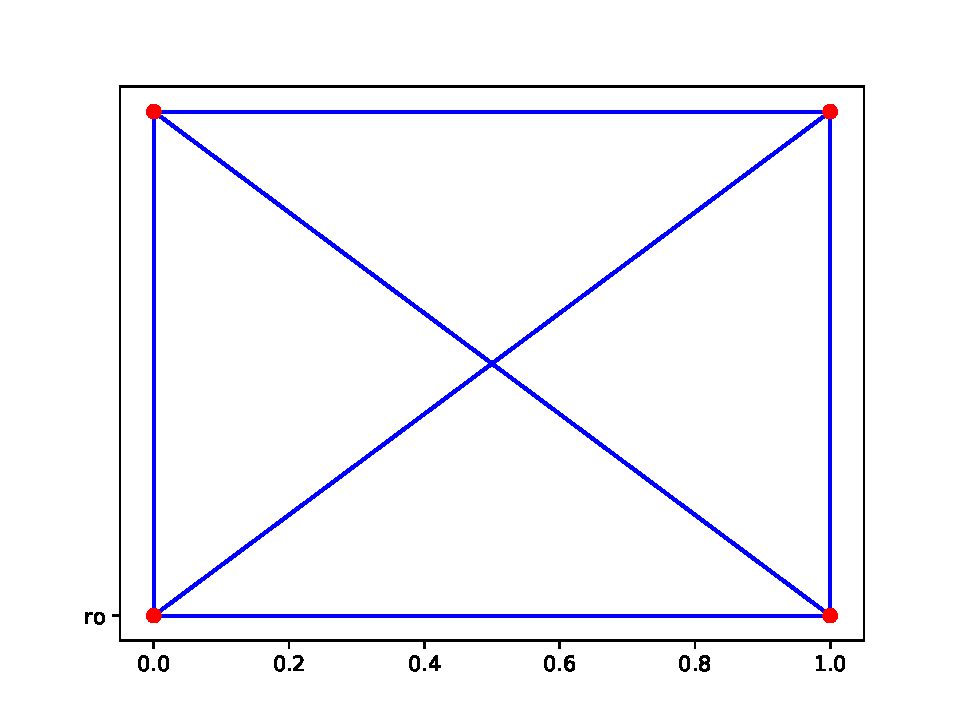
\includegraphics[width=0.45\linewidth]{./figs/square.pdf}
    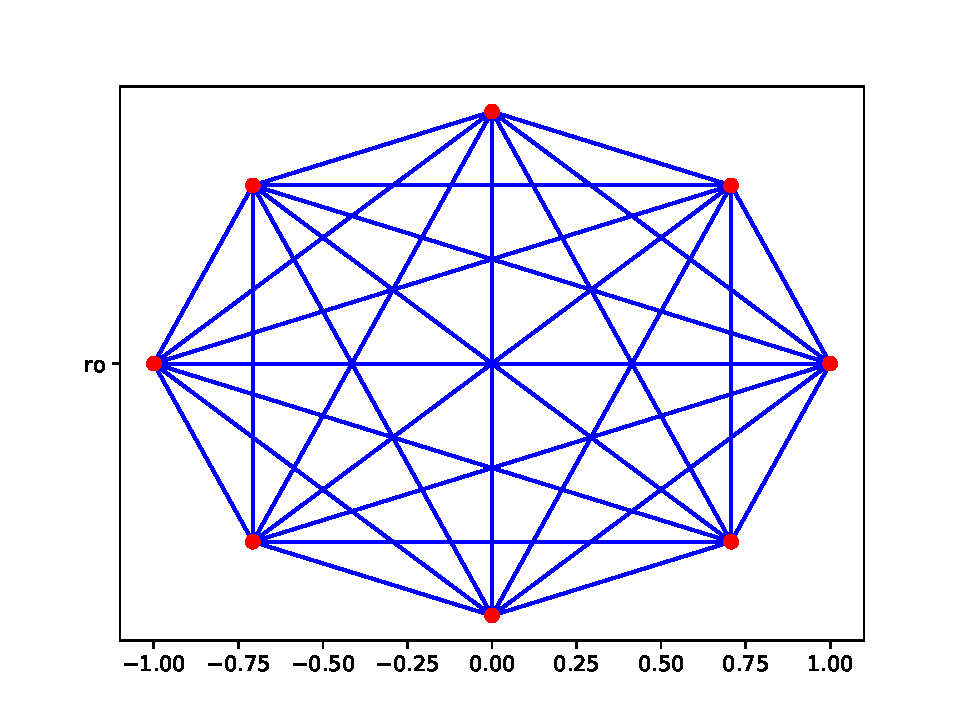
\includegraphics[width=0.45\linewidth]{./figs/circle.pdf}}
    \caption{Examples of complete graphs from Problem 5.14 b). The left shows the graph on the
    corners of the unit square, the right is the graph for eight equally spaced points on a circle.}
    \label{fig:graphs}
\end{figure}


\begin{Problem}{\textbf{Plotting graphs}}

\noindent Given a natural number $n$, make a function that plots the following graph:
\begin{itemize}
    \item Two vertical rows with $n$ points should be placed side by side.
    \item Each point on the left side should have a line to every point on the
    right side and vice versa.
    \item No two points on the same side should be connected by a single line.
\end{itemize}
Filename: \texttt{graph2.py}
\end{Problem}


\begin{Problem}{\textbf{Inefficiency of primality checker}}

\noindent Consider the program from Problem \ref{prime}. Use the \pythoninline{timeit} module and run the
program to find the time it takes to find a factorization of an $n$ digit number. Plot the time against
the number of digits for the numbers in the file \texttt{prime\_check.dat}.
You can use the following code to time the function for different numbers:
\begin{python}
str1 = "f(" + str(n) + ")"
str2= "g(" + str(n) + ")"
N = 100
time1 = timeit.timeit(str1, 'from __main__ import f',number=N)
time2 = timeit.timeit(str2, 'from __main__ import g',number=N)
\end{python}

Filename: \texttt{prime\_ineff.py}
\end{Problem}

\begin{Problem}{\textbf{Animating a cycloid}}

\noindent One may create a curve by placing a circle on the $x$-axis, fixing a point on the circle,
and then drawing the trace of the point as the circle is rolling. The resulting
curve is called a cycloid. In mathematical language it is given as
\begin{equation*}
    r(\theta) =[R(\theta-\sin\theta), R(1-\cos \theta)]
\end{equation*}
where $R$ is the radius of the rotating circle and $\theta$ is the angle starting
at 0 and increasing.

\paragraph{a)}
Animate the cycloid as a function of $\theta$ starting at 0, ending at 15. Draw
a point at the end of the cycloid that varies with the animation.

\emph{Hint: A point can be added through a new plot using for example} 
\newline
\pythoninline{point, = axes.plot([],[],'o')}

\emph{and updating during the animation.}

\paragraph{b)}
Add the rolling circle defining the cycloid to the plot. You may use that at a given
time $\theta$, the circle is given as $s(\theta)=(R\cdot\theta + \cos\theta, R + \sin\theta)$.

Filename: \texttt{cycloid.py}
\end{Problem}

\newpage
\begin{Problem}{\textbf{Calibration curve}}

\noindent
A tool in chemical analysis for measuring the concentration of a substance in a sample (e.g. blood or urine), is making a calibration curve. Solutions with known concentrations of a substance (standard solutions) are measured. The X-axis is the concentrations of the standard solutions, and the Y-axis is for the measured intensity of these solutions. The concentration of the substance in the sample can then be determined using an equation that best describes the calibration curve. This equation is determined using linear regression. 

In Python, you can use the \pythoninline{numpy} module to obtain a linear regression. How to do this will be shown.

Assume that you have made five standard solutions with concentrations of 10, 20, 30, 40 and 50 mg/L of the substance you wish to test for. You have used equipment that detects this substance, and noted down the intensity for each of your standard samples. The code below shows how the linear regression can be performed.
\begin{python}
# standard concentrations and height of their signals
I_stand = [9.19, 19.8, 27.0, 34.7, 44.9]
conc_stand = [10, 20, 30, 40, 50]

# linear regression
fit = np.poly1d(np.polyfit(conc_stand, I_stand, 1))
conc_curve = np.linspace(0, 60, 100)
signal_curve = fit(conc_curve)
\end{python}

\paragraph{a)} 
Plot the calibration curve as a line, and plot the intensities of the calibration solutions as points on top of the calibration curve. 

\paragraph{}
\noindent
The function created in the code above, \pythoninline{fit(x)}, is now a linear function on the form $f(x) = a x + b = y$, where $x$ corresponds to the concentration and $y$ will correspond to the intensity of the signal at the given concentration.

\paragraph{b)} 
Determine $a$ and $b$ by using \pythoninline{fit(x)} and use these to implement an inverse function of $f(x)$ such that $g(y) = x$. Use your function to calculate the concentration of three different samples of the same unknown compound. The intensities of the compound of the samples are given below.
\begin{python}
I_unknown = np.array([19.9, 20.1, 19.8])
\end{python}
Print out the mean value, with the uncertainty ($\overline{x} \pm s_N$), of the samples of the unknown compound. You may use \pythoninline{np.mean} and \pythoninline{np.std} to find the mean value and the uncertainty.

Filename: \texttt{calibration.py}
\end{Problem}
\chapter{Dictionaries and Strings}
%\section{Dictionaries and strings}

\begin{Problem}{\textbf{A result on primes ``dictionarized''}} \label{prob61}

\noindent Consider the program from Problem \ref{prob46}. Since the entries correspond to each other,
working with two seperate lists is cumbersome. We may avoid that using dictionaries.
Modify the program such that the values are saved in a dictionary instead of a list.
Let the values of $n$ be keys with values $\pi(n)$.

Filename: \texttt{primes\_dict.py}
\end{Problem}

\begin{Problem}\textbf{Chemical elements in a dictionary}
\noindent\\
Consider the dictionary \pythoninline{elements_10} consisting of the 10 first chemical elements of the periodic table:
\begin{python}
elements_10 = {1: '-', 2: 'Helium', 3: 'Lithium', 
         4: 'Beryllium', 5: 'Boron', 6: 'Carbon', 
         7: 'Nitrogen', 8: '-',
         9: 'Fluorine', 10: 'Neon'}
\end{python}
\paragraph{a)}
The chemical elements of number 1 (Hydrogen) and 8 (Oxygen) are missing. Copy \pythoninline{elements_10} into your file, and adjust the dictionary such that the keys 1 and 8 have their correct value. Use the technique as in this example:
\begin{python}
dictionary[key] = 'value'
\end{python}
\paragraph{b)} 
Copy the following code into your script, and run the file in your terminal. Find the difference between the two dictionaries that are printed, and explain why they are different from each other.
\begin{python}
elements_10_copy = elements_10.copy()
elements_10_copy.update({11: 'Sodium'})
print(elements_10)
print('\n')

elements_11 = elements_10
elements_11.update({11: 'Sodium'})
print(elements_10)
\end{python}

Filename: \texttt{chemical\_elements\_dict.py}
\end{Problem}
\newpage

\begin{Problem}{\textbf{Representation of polynomials}} \label{prob62}

\noindent Let $f(x)=\sum_{i=0}^n a_ix^i$ and $g(x)=\sum_{j=0}^mb_mx^m$ be two polynomials.
Recall that a polynomial can be expressed as a dictionary with keys equal to the
degree of a term, and the corresponding coefficient as value (so $3x^2+1/2$ is represented
by the dictionary $\{2: 3, 0: 1/2\}$). 

You will be asked to implement three functions in this exercise. Check that each of your functions work as expected by creating two different polynomials represented as dictionaries, call your functions and print the returned values.

\paragraph{a)}
Create a function that takes two dictionaries (corresponding to two polynomials
$f$ and $g$) as arguments and returns a dictionary corresponding to the sum of the two.

\paragraph{b)}
Create a function as above that returns the dictionary corresponding two the
product of two polynomials.

\emph{Hint: $fg=\sum_{k=0}^{n+m} c_kx^k$ where $c_k=\sum_{i+j=k}a_ib_j$}

\paragraph{c)}
Add a function that evaluates a polynomial dictionary at a point. 

Filename: \texttt{poly\_dict.py}
\end{Problem}

\begin{Problem} \textbf{Use string operations to create a pretty dictionary}

\noindent
The file \texttt{atm\_moon.txt} contains information about the composition of elements in the lunar atmosphere during nighttime. \cite{moon} The values are given in particles per cubic centimetre.


Write a function that reads the file, and returns a dictionary with the name of the element as keys and particle density as value. Transform all characters to their upper case equivalent. Strip off leading and trailing whitespaces in each of the string keys. Remove all the commas that marks every three digits, and then convert these values to float numbers.

For example, considering the information \pythoninline{' Neon 20 - 40,000 '} extracted from the file,
the value of the key \pythoninline{'NEON 20'} should look like this:
\begin{python}
'NEON 20': 40000
\end{python}

Filename: \texttt{atm\_moon.py}
\end{Problem}

\begin{Problem}{\textbf{Interpret output from a program}}

\noindent The program \texttt{approx\_derivative\_sine.py} calculates an approximation to the derivative of $\sin\left(\frac{\pi}{3} \right)$ by the expression
\begin{equation*}
    \frac{\partial f}{\partial x} \approx \frac{f(x + \Delta x ) - f(x)}{\Delta x} ,
\end{equation*}
for decreasing values of $\Delta x$. Direct the output of the program to a file (by \texttt{python approx\_derivative\_sine.py > filename}). Write a function that reads the file and returns three arrays consisting of numbers corresponding to \pythoninline{delta_x}, \pythoninline{abs_error} and \pythoninline{n}. Plot \pythoninline{delta_x} and \pythoninline{abs_error} versus \pythoninline{n}. Use a logarithmic scale on the $y$ axis. Explain why the absolute error increases after $n=8$, i.e. after \pythoninline{delta_x} = $10^{-8}$.


\emph{Hint: The function \pythoninline{semilogy} is an alternative to \pythoninline{plot} and gives logarithmic scale on the $y$ axis.}

Filename: \texttt{plot\_round\_off\_error.py}
\end{Problem}

\newpage
\begin{Problem}{\textbf{Saving information in a nested dictionary}}\label{prob63}

\noindent The file below contains information about various people. The first column is
the name, the second is the age, and the third is the gender.
\begin{lstlisting}
John, 55, Male
Toney, 23, Male
Karin, 42, Female
Cathie, 29, Female
Rosalba, 12, Female
Nina, 50, Female
Burton, 16, Male
Joey, 90, Male
\end{lstlisting}
\paragraph{a)}
Create a function that reads the file and returns the information in a nested
dictionary. For example the key 'John' has the dictionary
\{'Age': 55, 'Gender': 'Male'\} as value.
When reading the file, the name should read "John", not "John, ".
\paragraph{b)}
Create a function that takes as an argument a nested dictionary as above,
a person name, and optional arguments: a
number (age), and a string (gender) which returns the same dictionary with the new
age and gender. Note that neither should be changed if no age or gender is given.
\paragraph{c)}
Extend the function with the possibility to change the name of a person. One should
not be allowed to change a name to one that is taken (Can you think of a way
to allow this without overwriting another person?).
Read the file above and change the gender and name of John. Iterate the dictionary
and print the new information in a table format.
\begin{remark}
The nested dictionary here is a prototype of what is known as a class, and the
functions from b) is a prototype for what will be known as methods in that
class.
\end{remark}

Filename: \texttt{people\_dict.py}
\end{Problem}

\begin{Problem}{\textbf{Finding the frequency of words in a text}} \label{prob64}

\paragraph{a)}
Write a function that reads the file \emph{RandomWords.dat} and finds the frequency
of words of length $n$. Save the information in a dictionary with the length
as keys and the number of words of that length as values.  You may assume that
all words are separated by spaces and that only punctuation marks appear in the
text.

\emph{Hint: For your program to be compatible with words of any length, it might
be helpful to use defaultdict imported from collections. See page 339 in the book.
Use the function dict() on such an object to convert it to an ordinary dictionary}
\paragraph{b)}
Write a test function that generates a file of words and checks that the function
returns the correct values.

Filename: \texttt{word\_length.py}
\end{Problem}
\newpage 

\begin{Problem}{\textbf{The Euler's polyhedron formula}}
\noindent 
\\Let V, E, and F be the number of vertices, edges and faces in any polyhedron, respectively. Then, Euler's polyhedron formula tells us that
$$
V-E+F=2.
$$
In this exercise we shall check that the formula works for some given polyhedrons in a file with this setup:
\begin{lstlisting}
Polyhedron: cube
vertices: 8 edges: 12 faces: 6

Polyhedron: pyramid
vertices: 5 edges: 8 faces: 5

...
\end{lstlisting}

\paragraph{a)}
Write a function that can read such a file, and returns a dictionary with the type of the polyhedron as a key, and a dictionary containing vertices, edges and faces as a value. The function shall strip of leading and trailing whitespaces in all strings. For example, the value of the key \pythoninline{'cube'} in the dictionary should look like this:
\begin{python}
'cube': {'vertices': 8, 'edges': 12, 'faces': 6}
\end{python}
Note that you must convert the string numbers to integers, as for example $8$, not '$8$'. Be aware of the fact that the value of each polyhedron in the dictionary is again a dictionary. Print the (nested) dictionary that is returned when reading the file \texttt{polyhedrons.dat}.
\paragraph{b)}
Write a test function \pythoninline{test_polyhedron_formula()} that checks that Euler's polyhedron formula works for the polyhedrons given in \texttt{polyhedrons.dat}.\\
\noindent
\emph{Hint: Repeated indexing works for nested dictionaries as for nested lists. Below is an example of how to access the value of the key \pythoninline{'vertices'} inside the value of the key \pythoninline{'cube'}.}
\begin{python}
cube_vertices = polyhedrons_dict['cube']['vertices']
\end{python}

Filename: \texttt{polyhedron\_formula.py}

\end{Problem}
\newpage

\begin{Problem}{\textbf{Compute digital roots}}

\noindent Given a number, say 5282, we can compute the sum of the digits. In this case
$5+2+8+2=17$, and doing this again gives $1+7=8$. The one digit number we get by
doing this is called the digital root of the number.

\paragraph{a)}
Make a function that calculates the digital root of a number. 

\emph{Hint: Convert the number to a string in order to work with it.}

\paragraph{b)}
Plot the digital root of numbers up to 500 with the digital root on the $x$-axis and
the frequency of digital roots on the $y$-axis. Use \pythoninline{plt.scatter(x,y)} for the plot.

Filename: \texttt{dig\_root.py}
\end{Problem}



\begin{Problem}{\textbf{Timezone converter}}

\noindent In the file \texttt{timezones.dat} you will find places and their timezone in
GMT format.

\paragraph{a)}
Make a function that reads the file and saves the information in a dictionary.

\paragraph{b)}
Create a function that takes local Norwegian time (GMT +1) in the string format
'ddmmyy-hhmm', a place, and returns the local time at that place. Your program
should display a message to the user if a place that is not saved in the
dictionary is used. Do the following conversions:
\begin{itemize}
    \item March 21st 2018 05.34 in Vancouver
    \item December 31th 2017 20.03 in Sydney
    \item January 1st 2018 00.15 in London
\end{itemize}

Filename: \texttt{timezones.py}
\end{Problem} 


\chapter{Introduction to Classes}
%\section{Introduction to classes}

\begin{Problem}{\textbf{Saving information in a class}} \label{prob71}

\noindent In this problem you can use the program from \ref{prob63}.

\paragraph{a)}
Create a class \pythoninline{Person} where the constructor takes name, age, and gender as arguments.

\paragraph{b)}
Add methods to the class for changing a persons name, age, and gender.

\paragraph{c)}
Add a method \pythoninline{__str__} that returns a string with all the information of that person. Create an instance of the class, using the
information for 'John' in the table from Problem \ref{prob63}.
Change the name and gender of John. Print the information of the instance before and after changing.

Filename: \texttt{class\_people.py}
\end{Problem}


\begin{Problem}{\textbf{Right triangle class}}
\paragraph{a)}
Make a class \pythoninline{RightTriangle} that represents a right triangle. The constructor \pythoninline{__init__} should take and store two numbers $a$ and $b$. These are the two catheti (shortest sides) that define the right triangle. The constructor should also calculate and store the hypotenuse as a local variable in the class.

Remember that the hypotenuse $c$ relates to the two short sides $a$ and $b$ by the Pythagorean Theorem:
\begin{equation*}
    a^2 + b^2 = c^2
\end{equation*}

\paragraph{b)}
Make an object \pythoninline{triangle1} of the class  \pythoninline{RightTriangle} with both short sides equal to 1. Make another object \pythoninline{triangle2} with sides equal 3 and 4. Check that your implementation is correct by printing the hypotenuse of both objects. Use the usual \texttt{object.variable} convention to get the hypotenuse. 

\paragraph{c)}
To make a robust program, we often want to code it such that it prevents being used in ways that does not make sense. In our case, a natural thing to prevent is making a triangle with sides having negative length, since length is strictly positive.


Make changes to your class such that \pythoninline{ValueError} is raised if someone tries to make a triangle with sides of negative length.
To test that your class raises the error correctly, you can test it with the following code:

\begin{python}
def test_RightTriangle():
    success = False
    try:
        triangle3 = RightTriangle(1,-1)
    except ValueError:
        success = True
    assert success
\end{python}

\paragraph{d)}
Add a method \pythoninline{plot_triangle()} to your class which plots the triangle when you call it. The corner where the two shortest sides meet should be in origin. Side $a$ should be along the x-axis, and side b along y. In order to plot, you might want to find out what the coordinates of each corner must be. Also make sure to make the axis equally long so that the triangle looks nice (you can use \pythoninline{plt.axis("equal")}. Call the plotting method on the instance \pythoninline{triangle2} that you created in b).

Filename: $\texttt{right\_triangle.py}$
\end{Problem}


\begin{Problem}{\textbf{Make a function class}}

In this problem you will implement a \pythoninline{class F} which represents the function
\begin{equation*}
    f(x; n, m) =  \sin(n x) \cos(m x).
\end{equation*}

Create the class and let $n$ and $m$ be parameters of the constructor, which must be stored in the class.  


Since the class represents a function, it should be a callable class. An instance of a callable class can be called on like a function. The special method for creating a callable class is \pythoninline{__call__(self, args)}. Implement the special method \pythoninline{__call__(self, x)} such that it returns the value of the function evaluated at \pythoninline{x}. 

Create two different instances \pythoninline{u} and \pythoninline{v} of \pythoninline{class F}. Choose values $n$ and $m$ for both the instances. Plot the two instances \pythoninline{u} and \pythoninline{v} evaluated in $x$ against each other on the interval $x \in [0, 2 \pi]$. In other words, plot \pythoninline{u(x_values)} on the $x$-axis and \pythoninline{v(x_values)} on the $y$-axis. Make sure to have enough points on the interval to ensure that the line is smooth.


Filename: \texttt{F.py}
\end{Problem}

\begin{Problem}{\textbf{Extending the \pythoninline{AccountP} class}} \label{prob75}

\noindent Modify the class \pythoninline{AccountP} in the book to include a method \pythoninline{transfer} that transfers an amount between two accounts. The method should take an amount and the account you want to transfer to as arguments. Write a test function that checks that the methods \pythoninline{deposit}, \pythoninline{withdraw}, \pythoninline{transfer} and \pythoninline{get_balance} works properly.

Filename: \texttt{AccountP.py}

\end{Problem}

\newpage
\begin{Problem}{\textbf{Approximating the square root of two}} \label{prob72}

\noindent The square root of two can be represented by a so called \emph{continued fraction}
on the following form:
\begin{align*}
\sqrt(2)&= 1 + \frac{1}{1+\sqrt(2)} \\
        &= 1 + \frac{1}{2+\frac{1}{1+\sqrt(2)}} \\
        &= 1 + \frac{1}{2+\frac{1}{2+\frac{1}{1+\sqrt(2)}}}
\end{align*}
In this exercise we will exhibit two possibilities for approximating the number
$\sqrt(2)$.

\paragraph{a)}
Make a class \pythoninline{Square} with a method \pythoninline{approx_frac} that takes an integer $n$,
an initial value and returns the first $n$ fractions as above with initial value $x_0$. This can be done by iterating the
function
\begin{equation*}
    f(x) = 1+\frac{1}{1+x}
\end{equation*}
starting at $x_0$. For $n=2$ and $x_0=1$ this gives
\begin{equation*}
f(f(x_0)) = 1 + \frac{1}{2+\frac{1}{1+1}}.
\end{equation*}

\paragraph{b)}
Another way to approximate the square is by iterating the function $f(x)=\frac{1}{2}\left(x+\frac{2}{x}\right)$.
Add a method \pythoninline{approx_iter} that takes
a number $x_0$, an integer $n$, and 
returns the value of the function at $x_0$ iterated n times. For $n=2$ we would have
$f(f(x_0))$. From here on we assume for simplicity that $0.1 \leq x_0 \leq 2$.

\paragraph{c)}
Create a method that returns a nicely formatted table with
the two approximations and their difference $\epsilon$ along with the exact value for $n=1,2,5,10$.
Run the program, which approximation is best?

\paragraph{d)}
To visualize the approximation plot the exact value as a line in the plane
and the two approximations as points $(n, y_n)$, where $y_n$ is the approximation. Use $n = 1,2,5,10$.

Filename: \texttt{square\_iteration.py}
\end{Problem}

\begin{Problem}{\textbf{Tangent lines on a quadratic curve}} \label{prob73}

\noindent Consider a quadratic polynomial on the form $f(x)=x^2+bx+c$. At a point $x_0$ the
tangent line is given by $l(x)=(2x_0+b)x +C$ where $C=f(x_0)-(2x_0+b)x_0$.
\paragraph{a)}
Make a class \pythoninline{Quadratic} with a function $f(x)$ (a quadratic polynomial as above) as initial
argument. Make a method that computes the tangent at a point and returns the function
$l(x)$.

\emph{Hint: You will need to extract the coefficients $b=f(1)-f(0)-1$ and
$c=f(0)$.}
\paragraph{b)}
Create a method that plots the function along with its tangent at a point.
\paragraph{c)}
Make a method that animates the tangent line moving over the curve $f(x)$. Make
the animation for uniformly distributed x values in the interval $-5 \leq x \leq 5$.
Test the program with the function $f(x)=x^2$.

Filename: \texttt{quadratic\_tangents.py}
\end{Problem}


\begin{Problem}{\textbf{Numerical approximations for the derivative}} \label{prob74}

\noindent Let $f(x)$ be a function and $f'(x)$ its derivative. There are many ways to
approximate the derivative, some of which are:
\begin{align*} 
    f'(x) &\approx  \frac{f(x+h)-f(x)}{h} \\
    f'(x) &\approx  \frac{f(x+h)-f(x-h)}{2h} \\
    f'(x) &\approx  \frac{-f(x+2h)+8f(x+h)-8f(x-h)+f(x-2h)}{12h}
\end{align*}
\paragraph{a)}
Make a class \pythoninline{Diff} with a function $f$ as initial argument and implement
three methods \pythoninline{diff1}, \pythoninline{diff2}, and \pythoninline{diff3}
approximating the derivative using the above formulas.


\paragraph{b)}
Create an instance of the class \pythoninline{Diff}, using $f(x) = \sin\left( 2 \pi x \right)$. Visualise the difference in accuracy of the three methods for computing the derivative by comparing the results with the exact function for the derivative, $f'(x) = 2 \pi \cos(2 \pi x)$. Use the four values  $h = 0.9, 0.6, 0.3, 0.1$, and let $x$ be on the interval $x \in [-1, 1]$. 

Filename: \texttt{class\_diff.py}
\end{Problem}

\begin{Problem}{\textbf{Visualizing functions}}

\noindent For a function $f(x)$ we can plot the graph of the function as points $(x,f(x))$.
This results in a curve in the plane. Suppose we have a function
 \begin{equation*}
 f(x,y)=(u(x,y),v(x,y)).
 \end{equation*}
The graph of this function lives in four dimensions and is not easily visualized.
On way to visualize these functions is to instead of looking at the graph we look
at how $f$ act on points. For example, how the grid lines in the plane look
after $f$ is applied.

\paragraph{a)}
First we consider a specific function $f(x,y)=(x^2-y^2,2xy)$.
Write a program where you define the function $f$
and make a figure with $x$ and $y$ axis from -2 to 2 where you plot a number of
the grid lines in $x$ and $y$ direction in the same plot. You will need around 15 lines
in each direction. Make a another plot side-by-side in the same figure of all points
$(x^2-y^2,2xy)$ where $x$ and $y$ are the points in the first plot.

\paragraph{b)}
To make the construction more flexible, modify your program to be a class \pythoninline{Visualize} taking
a function $f(x,y)=(u(x,y),v(x,y))$ as initial argument. It should contain
a method \pythoninline{grid(self, n)} that generates two plots, one of grid lines,
and one of the image as in a).

\paragraph{c)}
We used grid lines of the plane to see how the function $f$ behaved. We could have
used any curves in the plane. Extend the class with a method \pythoninline{circ} that instead of using
points corresponding to grid lines, uses circles with expanding radii. Let the
axes go from -5 to 5 and the radii be uniformly distributed between
0 and 10 (15 circles should be sufficient). Test with the function $f(x,y)=(x^2-y^2+x+1,2xy+y)$.
The second plot should consist of circular like objects with a self-crossing.

\paragraph{d)}
Add a method \pythoninline{grid_anim} that shows an animation of the image of the
functions
\begin{equation*}
    f_\epsilon(x,y)=[(1-\epsilon) x + \epsilon u(x,y), (1-\epsilon)y-\epsilon v(x,y) ]
\end{equation*}
where $\epsilon$ varies from 0 to 1.

\paragraph{e)}
Using the functions
\begin{align*}
    f(x,y)=(x^2-y^2, 2xy) \quad \text{and} \quad g(x,y)=(x^2-y^2+x+1,2xy+y),
\end{align*}
test the \pythoninline{grid} and \pythoninline{grid_anim} methods on $f$, and the \pythoninline{circ} method on $g$. Use 15 gridlines
and 15 circles.
\begin{remark}
For the student familiar with complex numbers, this is exactly how one would
visualize a complex function $f(z)$. In our case we can use this for any function
$f(x,y)$, but we usually restrict ourself to look at functions corresponding to
certain complex functions, namely the differentiable ones.
\end{remark}

Filename: \texttt{plot\_functions.py}
\end{Problem}


\begin{Problem} {\textbf{A class for coordinates}}

\noindent
This exercise will focus on how to implement special methods. You will implement the class \pythoninline{Coords}, which represents coordinates in three dimensions. 

\emph{Hint: the class of complex numbers shown in the book is of similar nature to the class you should implement in this problem.}



\paragraph{a)} Create the class \pythoninline{Coords}. Start by implementing the special methods \pythoninline{__init__(self, args)} and \pythoninline{__str__(self)}.  The constructor should take three parameters, $x$, $y$ and $z$. The representation of the class should be $(x, y, z)$.

The implementation should be such that the code below works.
\begin{python}
sqrt3 = sqrt(3)
close = Coords(1/sqrt3, 1/sqrt3, 1/sqrt3)
far = Coords(3/sqrt3, 15/sqrt3, 21/sqrt3)

print("The coordinates close are at %s" %close)
print("The coordinates  far  are at %s" %far)
\end{python}
Output:
\begin{lstlisting}
The coordinates close are at (0.58, 0.58, 0.58)
The coordinates  far  are at (1.73, 8.66, 12.12)
\end{lstlisting}


\paragraph{b)} Implement the special methods \pythoninline{__len__(self)} and \pythoninline{__abs__(self)}. The length of coordinates should always be 3, as the coordinates will be in three dimensions. The absolute value should yield the Euclidean norm (or the physical length in space), which is given by
\begin{equation*}
    ||(x, y, z)||= \sqrt{x^2 + y^2 + z^2} .
\end{equation*}

The implementation should be such that the code below works.
\begin{python}
print("The class Coords represents coordinates in \
%d dimensions" %len(close))

print("\nThe distance from the centre to the point \
close is %.2f" %abs(close))
print("The distance from the centre to the point  \
far  is %.2f" %abs(far))
\end{python}
Output:
\begin{lstlisting}
The class Coords represents coordinates in 3 dimensions

The distance from the centre to the point close is 1.00
The distance from the centre to the point  far  is 15.00
\end{lstlisting}


\paragraph{c)} Implement the special methods \pythoninline{__add__(self, other)} and \newline  \pythoninline{__sub__(self, other)}. When adding or subtracting two objects of class \pythoninline{Coords}, a new object of class \pythoninline{Coords} should be returned. 

The object returned when adding two coordinates should have the coordinates
\begin{equation*}
\begin{split}
    x_{new} &= x_{self} + x_{other} \\
    y_{new} &= y_{self} + y_{other} \\
    z_{new} &= z_{self} + z_{other} ,
\end{split}
\end{equation*}
and similarly should the method for subtracting should return an object of \pythoninline{Coords} with coordinates at
\begin{equation*}
\begin{split}
    x_{new} &= x_{self} - x_{other} \\
    y_{new} &= y_{self} - y_{other} \\
    z_{new} &= z_{self} - z_{other} ,
\end{split}
\end{equation*}

The implementation should be such that the code below works.
\begin{python}
further = close + far
print("The coordinates further are at %s" %further)

distance = abs(far - close)
print("\nThe distance from far to close is %.2f" %distance)

centre = further - further
print("\nThe coordinates at the centre are %s" %centre)
\end{python}
Output:
\begin{lstlisting}
The coordinates further are at (2.31, 9.24, 12.70)

The distance from far to close is 14.14

The coordinates at the centre are (0.00, 0.00, 0.00)
\end{lstlisting}


Filename: \texttt{Coords.py}
\end{Problem}

\chapter{Random Numbers and Simple Games}
%\section{Random numbers and simple games}

\begin{Problem}{\textbf{Throw a die}}
%\addcontentsline{toc}{section}{Exercise 8.1: Throw a die - \texttt{die.py}}

\noindent Compute the probability of getting a $6$ when throwing a die. Write a program
that throws a die $N$ times and count how many times the die shows $6$, let this
number be $M$. Then compute the probability of getting a $6$ when throwing a die
as $M/N$.

Filename: $\texttt{die.py}$
\end{Problem}

\begin{Problem}{\textbf{Telephone number}}
%\addcontentsline{toc}{section}{Exercise 8.2:  - \texttt{telephone.py}}

\noindent A Norwegian telephone  number consists of eight digits. We assume that all digits
from $0$ to $9$ are equally probable in every place of the telephone number.
Make a program that finds the probability of having a telephone number where the
digit $1$ appears at least four times.

Filename: $\texttt{telephone.py}$
\end{Problem}

\begin{Problem}{\textbf{Coin-flip game}}
%\addcontentsline{toc}{section}{Exercise 8.3: Coin-flip game - \texttt{coin.py}}

\noindent Two persons are playing a simple coin-flip game. They flip a coin in turn,
and whoever first gets a heads wins the game. Make a program to model $100$ such
games. Estimate the probability for the first person to flip to win the game.

Filename: $\texttt{coin.py}$
\end{Problem}

\begin{Problem}{\textbf{Birthday probability}}

\noindent Make a function that generates a string of random integers between 0 and 9.
Estimate the probability that your birthday is contained in a string of random
numbers of length 1000. Let the format of the date be on the form \pythoninline{ddmmyy}.
Print the estimates in \%.

Filename: \texttt{birthday\_prob.py}
\end{Problem}
\newpage

\begin{Problem}{\textbf{Approximate $\pi$ by throwing darts}}
%\addcontentsline{toc}{section}{Exercise 8.4: Approximate $\pi$ by throwing darts - \texttt{approximate\_pi.py}}

\noindent You are throwing darts at a square shaped target with an inscribed circle. Let
the length of the sides of the square be $2$, which means that the circle has
radius $1$. Assume that you throw the darts such that the darts gets uniformly
distributed on the target. Then, the number of darts which hits the target inside
the circle divided by the total number of darts that hits the target is
approximately the area of the circle divided by the total area of the target.
This approximation gets more accurate the more darts you throw.
\begin{equation*}
\frac{\mathrm{number\; of\; darts\; inside\; circle}}
{\mathrm{number\; of\; darts\; that\; hits\; target}}
\approx \frac{\mathrm{area\; of\; circle}}{\mathrm{area\; of\; target}}
= \frac{\pi}{4}.
\end{equation*}
Thus, $\pi$ can be approximated by
\begin{equation*}
\pi \approx 4 \frac{\mathrm{number\; of\; darts\; inside\; circle}}
{\mathrm{number\; of\; darts\; that\; hits\; target}}.
\end{equation*}
Write a program that throws $M$ darts uniformly on the target. Then approximate
$\pi$. Read $M$ from the command line.

Filename: $\texttt{approximate\_pi.py}$
\end{Problem}

\begin{Problem}{\textbf{Wheel of fortune}}
%\addcontentsline{toc}{section}{Exercise 8.5: Wheel of fortune - \texttt{wheel\_of\_fortune.py}}

\noindent At an amusement park they have a wheel of fortune where you can win $2$kg of
chocolate. You get to choose one number between $1$ and $20$ for $20$NOK. Assume that you
play on the same number until you win.

\paragraph{a)}
Write a program that finds the average number of times you have to play before
you win and check if you earn or loose money, compared to buying 2kg of chocolate in the store.

\paragraph{b)}
Modify your program so that every time you lose you move one place to the right,
i.e. you increase $n$ by one. If you are at $n = 20$ you go back to $n = 1$.
Does this make any difference to the result?

Filename: \texttt{wheel\_of\_fortune.py}
\end{Problem}

\chapter{Object-Oriented Programming}
%\section{Object oritented programming}

\begin{Problem}{\textbf{Implement Newtons method}} \label{prob91}

\paragraph{a)}
Make a subclass \pythoninline{Function} of the class \pythoninline{Diff} in problem \ref{prob74}
that takes a function $f$ as
an initial variable. It should contain a method such that the following code
is compatible with your program and prints the value of $f$ at 2.
\begin{python}
def f(x):
    return x**2
func = Function(f)
print(f(2))
\end{python}

\paragraph{b)}
We would like the class to give estimated values for roots of $f$. That is,
points such that $f(x)=0$. To do this we implement Newton's formula. It is given
recursively as
\begin{equation*}
    x_{n+1}=x_n-\frac{f(x_n)}{f'(x_n)},
\end{equation*}
where we give a starting point $x_0$. In some cases(not all) $x_n$ will approach
a root of $f$. Implement this in a method \pythoninline{approx_root} that takes a
starting point and a bound $\epsilon<1$ as arguments and approximates $x_n$ such that
$f(x_n)<\epsilon$.

\emph{Hint: Implement a simple convergence test. Check that $f(x_n)<1$ after $100$ iterations. If
not terminate the loop and inform the user that there is no convergence for that
starting point. It is still a possibility for convergence, but unlikely.}

\paragraph{c)}
Test the program with the function $f(x)=x^2-1$ and starting value 5 with bounds
$10^{-i}$, for $i=1,2,3,4,5,6$. Print the approximated value for $x$, $f(x)$ and the
bound in a table format. Try to run the program with starting value 0. What happens,
can you see why?

Filename: \texttt{newton.py}
\end{Problem} 

\newpage
\begin{Problem}{\textbf{Implement Polynomials as a Class}} \label{prob92}

\paragraph{a)}
Make a class Quadratic that implements second order polynomials. An object of Quadratic should be initialised with a list containing the coefficients. Add a \pythoninline{__call__}-method that evaluates the parabola at a point \pythoninline{x}, and a \pythoninline{__repr__}-method such that you can print your polynomial.
\\
Make an object of Quadratic with coefficients $(1, 3, 2)$. Print it and evaluate it at $x=1$, $x=2$ to make sure it works.   

\paragraph{b)}
Make a subclass Cubic of the class Quadratic that implements third order polynomials. You should make use of inheritance to extend the class Quadratic you made in the previous exercise. Implement a method \pythoninline{derivative} for Cubic. The method should return an object of type Quadratic that corresponds to the derivative.
\\
Make an object of Cubic with coefficients $(1, 3, 2, 4)$. Print it and evaluate it at $x=1$, $x=2$. Also call \pythoninline{derivative} and print the result.

Filename: \texttt{polynomial.py}
\end{Problem} 

\begin{Problem}{\textbf{Vectors}} \label{prob93}

\paragraph{a)}

Make a class Vector2D that implements 2D-vectors(two components). Add \pythoninline{__add__} and \pythoninline{__sub__} methods so you can add and subtract vectors. Remember that vectors add and subtract element-wise, e.i.:
\begin{equation*}
    (1,2) + (4,5) = (5,7) 
\end{equation*}

\paragraph{b)}
For two vectors $\Vec{a} = (a_1, a_2)$ and $\Vec{b} = (b_1, b_2)$, the dot product is defined as 
\begin{equation*}
    \Vec{a} \cdot \Vec{b} = a_1 b_1 + a_2 b_2
\end{equation*}
\\
Implement a method \pythoninline{dot} that calculates the dot product of two vectors.
\\
Make two vectors $\Vec{v}=(1,2)$ and $\Vec{w}=(-2,5)$ from Vector2D. Print $\Vec{v}$, $\Vec{w}$, $\Vec{v}+\Vec{w}$, $\Vec{v}-\Vec{w}$ and $\Vec{v}\cdot \Vec{w}$

\paragraph{c)}
Make a subclass Vector3D of the class Vector2D, where Vector3D is extended with an additional coordinate. Make sure all the methods are updated to work with three coordinates. The dot product for 3D vectors extends as one would expect:

\begin{equation*}
    \Vec{a} \cdot \Vec{b} = a_1 b_1 + a_2 b_2 + a_3 b_3
\end{equation*}
Use inheritance to reuse old code as much as possible(especially for the dot product method).
\\
Make two vectors $\Vec{v}=(1,2,4)$ and $\Vec{w}=(-2,5,1)$ from Vector3D. Print $\Vec{v}$, $\Vec{w}$, $\Vec{v}+\Vec{w}$, $\Vec{v}-\Vec{w}$ and $\Vec{v}\cdot \Vec{w}$

\paragraph{d)}
There is a common vector operation that is defined for 3D vectors, but not for 2D vectors. This is the cross product. It differs from the dot product in that the result is not a number, but a new vector:
\begin{equation*}
    \Vec{c} = \Vec{a} \times \Vec{b}
\end{equation*}
where $\Vec{c} = (c_1, c_2, c_3)$. The cross product is define as
\begin{align*}
    c_1 = a_2 b_3 - a_3 b_2\\
    c_2 = a_3 b_1 - b_1 a_3\\
    c_3 = a_1 b_2 - b_2 a_1\\
\end{align*}
Implement a method \pythoninline{cross} for Vector3D only that calculates the cross product. \\
Make two vectors $\Vec{v}=(2,0,0)$, $\Vec{w}=(0,2,0)$ from Vector3D. Print $v\times w$.
\\
Filename: \texttt{vector.py}
\end{Problem}

\begin{Problem}{\textbf{Inheritance}} \label{prob94}
\\
In this exercise we will investigate how python handles inheritance by making some intuitive classes. 

\paragraph{a)}
Begin by making a class \pythoninline{Mammal}. Add a method \pythoninline{info()} that returns a string stating something that is common among all mammals, e.i. "I have hair on my body". Also add a method \pythoninline{identity_mammal()} that prints "I am a mammal".

\paragraph{b)}
Make a subclass Primate of the class Mammal. Add a method \pythoninline{info()} that returns the same as \pythoninline{info()} for Mammal, in addition to something new specific for Primates. E.i. "I have a large brain". Do not include the string from Mammal by copy-pasting, but use inheritance. Also add a method
\pythoninline{identity_primate()} equivalent to \pythoninline{identity_mammal()}.

\paragraph{c)}
Now make two subclasses Human and Ape from Primate. Update \pythoninline{info()} in the same manner for both Human and Ape, and also add their respective identity method.


Make an object John of the class Human, and an object Julius of the class Ape. Try calling \pythoninline{info()}, \pythoninline{identity_mammal()},   \pythoninline{identity_primate()},  \pythoninline{identity_human()} and \pythoninline{identity_ape()} for both John and Julius. Does it work as you expect? Some of these calls are meant to cause an error. 
\paragraph{d)}
Python is able to check if an object is of a particular class with the function \pythoninline{isinstance}. 
\pythoninline{isinstance(object_name, class_name)} returns \pythoninline{True} if the object \pythoninline{object_name} is of class \pythoninline{class_name}. An example could be   
\pythoninline{isinstance(John, Primate)}, which returns \pythoninline{True} if John is of the class Primate.


Use \pythoninline{isinstance} to check if John is Mammal, Primate, Human and Ape. Do the same for Julius.

Filename: \texttt{inheritance.py}
\end{Problem}

\appendix
\chapter{Sequences and Difference Equations}
%\section{Sequences and difference equations}
The exercises of this chapter correspond to Appendix A in the book by Langtangen,
and cover programming of difference equations.

\begin{Problem}{\textbf{Computing Bell numbers}}

\noindent Let $B_0=B_1=1$, the $n$'th \emph{Bell number} is defined recursively as
\begin{equation*}
    B_{n+1}=\sum_{k=0}^n \binom{n}{k}B_k.
\end{equation*}
Make a function that returns the $n$ first Bell numbers and print the first 10.

Filename: $\texttt{bell.py}$
\end{Problem}

\begin{Problem}{\textbf{Solve a difference equation numerically}}
%\addcontentsline{toc}{section}{Exercise A.1: Solve a difference equation numerically  - \texttt{fibonacci.py}}

\noindent We study the difference equation
\begin{equation*}
x_n = x_{n-1} + x_{n-2}.
\end{equation*}
Write a program that writes out the first $15$ elements of the sequence for $x_0 = x_1 = 1$.

Filename: $\texttt{fibonacci.py}$
\end{Problem}


\begin{Problem}{\textbf{The spreading of a disease}}
%\addcontentsline{toc}{section}{Exercise A.2: The spreading of a disease  - \texttt{disease.py}}

\noindent We want to study the spreading of a disease. Assume that people recover at a rate such that a ratio $a$ of the people
that are sick this week will still be sick next week. It takes two weeks from when you
get infected until you become sick, and a person who is sick will on average infect
$b$ people each week, who then become sick two weeks later.

Let $x_n$ be the
number of sick people in week $n$. The number of sick people is then given by the following difference equation
\begin{equation*}
x_n = a x_{n-1} + b x_{n-2} .
\end{equation*}

\paragraph{a)}
Write a function \pythoninline{disease_weeks(a, b, x0, x1, N)} that calculates the number of people that are ill with a given disease (defined by values $a$ and $b$) and returns an array/list containing the number of sick people form the initial week to week $N$. (In other words, the function should return an array or a list with $x_0, x_1, ..., x_N$).

Let  $x_0 = 100$ , $x_1 = 150$ and $a = 0.25$. Use the function calculate the number of sick
people in an array up to week $N = 15$ for both $b = 0.5$ and $b = 0.75$. Plot both scenarios in the same plot. Remember to use labels on the curves.


\paragraph{b)}
We do not need to store all the $N + 1$ values. Since $x_n$ only depends on
$x_{n-1}$ and $x_{n-2}$, these are the only values we need to store. Write a function \pythoninline{disease_week_N(a, b, x0, x1, N)} that does not use any lists or arrays, and returns only the number of sick people in week $N$, $x_N$. Use this function to obtain the number of sick people in week $N = 15$ for both the cases you plotted in a). Print out the results, and remember to include information about which of the two cases you are printing. Verify that the result is the same as obtained using arrays.

Filename: $\texttt{disease.py}$
\end{Problem}

\begin{Problem} \textbf{{Finding $\pi$ with Newton's method}}

\noindent
It is common knowledge that $\pi \approx 3.14$, but in this exercise you will use Newton's method and knowledge of the sine function to improve an approximation of $\pi$.

Newton's method can be written as a difference equation defined \begin{equation*}
    x_n = x_{n - 1} - \frac {f(x_{n-1})} {f'(x_{n-1}) } ,
\end{equation*}
and is used to find roots of $f(x)$, based on the function $f(x)$, the derivative of the function $f'(x)$ and an initial guess $x_0$.

Consider the function $f(x) = \sin(x)$. Finding the functions derivative $f'(x)$, should be trivial. This function has infinitely many roots, which we know are located at $x = k \pi$, where $k$ is an integer. This exercise will focus on the root for $k = 1$, and use Newton's method to approximate $\pi$. For Newton's method to converge towards the correct root, the initial condition, $x_0$, needs to be set close to the value of $\pi$.
\bigskip

Set $x_0 = 3.14$ and calculate $x_1$ and $x_2$ following Newton's method. Print out $x_0$, $x_1$ and $x_2$, as well as the value of \pythoninline{numpy.pi} with 13 decimals. You should print them in a tidy way such that the values are easy to compare. If Newton's method was used correctly, your values for $\pi$ should improve!


Filename: \texttt{finding\_pi.py}
\end{Problem}


\begin{Problem}{\textbf{Find difference equations for computing $\ln x$}}
%\addcontentsline{toc}{section}{Exercise A.3: Find difference equations for computing $\ln x$  - \texttt{ln\_Taylor\_series\_diffeq.py}}

\noindent
The Taylor expansion of $\ln x$ is
\begin{equation*}
\ln x = \sum_{n = 1}^\infty (-1)^{n + 1}\frac{(x - 1)^ n}{n},
\end{equation*}
for $x \in (0, 2]$.

We can define the sum as
\begin{equation*}
\ln x \approx S(x; n) = \sum_{j = 0}^n (-1)^{j + 1}\frac{(x - 1)^ j}{j},
\end{equation*}
so that $S(x, n) = \sum_{j = 1}^n a_j$ and
\begin{equation*}
a_j = -\frac{(j-1)}{j}(x - 1)a_{j-1}.
\end{equation*}
Introduce $s_j = S(x, j - 1)$ and $a_j$ as the two sequences to compute. We have
the initial values $s_1 = 0$ and $a_1 = (x - 1)$.

\paragraph{a)}
Find the set of difference equations for $s_j$ and $a_j$.

\emph{Hint: You can find an example on how this is done for $e^x$ in
section A.1.8 in the book.}

\paragraph{b)}
Implement the system of difference equations in a function
\pythoninline{ln_Taylor(n, x)} which returns $s_{n + 1}$ and $\lvert a_{n+1}\rvert$.
The term $\lvert a_{n+1}\rvert$ is the first neglected in the sum and may act as a
rough estimate of the size of the error in the Taylor polynomial approximation.

\paragraph{c)}
Verify the implementation by computing the difference equations
for $n = 3$ by hand and comparing with the output from the \pythoninline{ln_Taylor}
function. Automate this comparison in a test function.

\paragraph{d)}
Check that the accuracy of the Taylor polynomial improves as $n$
increaces and $x$ is close to $1$. What happens when $x > 2$?

Filename: $\texttt{ln\_Taylor\_series\_diffeq.py}$
\end{Problem}

\begin{Problem}{\textbf{Lotka-Volterra two species model}}
%\addcontentsline{toc}{section}{Exercise A.4: Lotka-Volterra two species model  - \texttt{Lotka\_Volterra.py}}

\noindent We have previously studied the logistic model for poulation growth. This is a
model showing the growth of a population in the abscence of predators. The
Lotka-Volterra model describes interactions between two species in an ecosystem,
a predator and a prey. We will in the following take the preys to be rabbits and the
predators to be foxes. The number of rabbits and foxes in week $n$ is denoted by
$R_n$ and $F_n$ respectively, and the population is modelled by the equations
\begin{align*}
R_{n+1} &= R_n + aR_n - cR_nF_n\\
F_{n+1} &= F_n + ecR_nF_n - bF_n,
\end{align*}
where $a$ is the natural growth rate of rabbits in the absence of predation, $b$ is
the natural death rate of foxes in the absence of food (rabbits), $c$ is the death
rate per encounter of rabbits due to predation and $e$ is the efficiency of turning
predated rabbits into foxes.

Write a program that computes the number of rabbits and foxes up to $n = 500$.
Use $a = 0.04$, $b = 0.1$, $c = 0.005$ and $e = 0.2$. In the begining we have
$R_0 = 100$ and $F_0 = 20$. Plot how the number of individuals in the populations
vary with time.

Filename: \texttt{Lotka\_Volterra.py}
\end{Problem}

\begin{Problem}
{\textbf{Difference equations for computing arctan(x)}}

\noindent
The purpose of this exercise is to implement difference equations for computing a Taylor polynomial approximation to $\arctan(x)$. For $x \in (-1, 1)$, we have
$$
\arctan(x) \approx S(x;n) = \sum_{j=0}^{n}(-1)^j\frac{x^{2j+1}}{2j+1}.
$$
To compute $S(x;n)$ efficiently, we can write the sum as $S(x;n)=\sum_{j=0}^{n}a_j$, and derive a relation between two consecutive terms in the series:
$$
a_j = -x^2\frac{(2j-1)}{(2j+1)}a_{j-1}.
$$
We introduce $s_j=S(x;j-1)$ and $a_j$ as the two sequences to compute. We have $s_0=0$ and $a_0=x$.
\paragraph{a)}
Implement the system of difference equations in a function\\ \pythoninline{arctan_Taylor(x,n)}. The function shall not use any lists or arrays. (Since $a_j$ only depends on $a_{j-1}$, and $s_j$ only depends on $s_{j-1}$ and $a_{j-1}$, these are the only values that we need to store.) The function shall return $s_{n+1}$ and $|a_{n+1}|$. The latter is the first neglected term in the sum (since $s_{n+1}=\sum_{j=0}^{n}a_j$) and may act as a rough measure of the size of the error in the Taylor polynomial approximation.
\bigskip

The function \pythoninline{arctan_Taylor(x, n)} will give extremely inaccurate approximations to $\arctan(x)$ for $x\not\in (-1, 1)$. To find a good approximation to $\arctan(x)$ for all $x$, we can use the fact that
\begin{align*}
\arctan(x) =& \frac{\pi}{2} - \arctan \left(\frac{1}{x}\right)\\
\approx& \frac{\pi}{2} - S(x;n),
\end{align*}
for values of $x\geq1$.
\paragraph{b)}
Implement the following piecewise function as a python function\\ \pythoninline{arctan_Taylor_improved(x, n)}. Your function shall return both the approximation and the measure of the size of the error as in \pythoninline{a)}.


\[
  \arctan(x)\approx \left\{
     \begin{array}{@{}l@{\thinspace}l}
      \hspace*{2.7mm} \frac{\pi}{2} - S\left(\frac{1}{x};n\right)  \hspace*{17.5mm}  1 \leq x \\
        \hspace*{9.5mm}S\left(x;n\right) \hspace*{14.5mm} -1 < x < 1\\
       -\frac{\pi}{2} - S\left(\frac{1}{x};n\right)  \hspace*{13.5mm} -1 \geq x \\
     \end{array}
   \right.
\]
\emph{Hint: Call the function \pythoninline{arctan_Taylor} inside the piecewise function.}
\paragraph{c)}
Write a test function to verify the approximation from \pythoninline{b)}. Test for $x=[-4, -0.5, 0.7, 10]$ with $n=10$, and with tolerance $=10^{-5}$.

\paragraph{d)}
Make a table or plot of the approximation from \pythoninline{b)} for various $x$ and $n$ to illustrate that the accuracy improves as $n$ increases.


In the table; include the $x$ value and the order $n$, the approximation and the exact value, and the measure of the error.


In the plot; calculate for $x\in[-20, 20]$. Include also the exact function for comparison, and remember to label the graphs.



Filename: \texttt{arctan\_Taylor\_series\_diffeq.py}
\end{Problem}


\addtocounter{chapter}{3}
\chapter{Programming of Differential Equations}
%\section{Programming of differential equations}
The exercises of this chapter are about programming of solvers for ordinary differential
equations, corresponding to Appendix E in the book by Langtangen.


\begin{Problem}{\textbf{Solve a simple ODE with function-based code}}\label{simple_ode_func}

\noindent
This exercise aims to solve the ODE problem $u - 5u' = 0, u(0) = 0.1$, for $t \in [0,20]$.
\paragraph{a)} Identify the mathematical function $f(u,t)$ in the generic ODE form $u' = f(u,t)$.
\paragraph{b)} Implement the $f(u,t)$ function in a Python function.
\paragraph{c)} Use the \pythoninline{ForwardEuler} function from Section 2.1 of the
lecture notes \emph{Solving Ordinary Differential Equations in Python} to compute a numerical solu-
tion of the ODE problem. Use a time step $\Delta t = 5$.
\paragraph{d)} Plot the numerical solution and the exact solution $u(t) = 0.1e^{0.2t}$.
\paragraph{f)} Perform simulations for smaller $\Delta t$ values and demonstrate visually that the
numerical solution approaches the exact solution.

Filename: \texttt{simple\_ODE\_func.py}
\end{Problem}

\begin{Problem}{\textbf{Solve a simple ODE with class-based code}}\label{simple_ode_class}

\noindent
Solve the same ODE problem as in Exercise \ref{simple_ode_func}, but use the
\pythoninline{ForwardEuler} class described in Section 2.2 of the lecture
notes \emph{Solving Ordinary Differential Equations in Python}.
Implement the right-hand side function $f$ as a class too.

Filename: \texttt{simple\_ODE\_class.py}
\end{Problem}

\begin{Problem}{\textbf{Solve a simple ODE with the ODEsolver hierarchy}}

\noindent
Solve the same ODE problem as in Exercise \ref{simple_ode_func}, but use the
\pythoninline{ForwardEuler} class in the \pythoninline{ODESolver} hierarchy
from Section 2.4 of the lecture notes.

Filename: \texttt{simple\_ODE\_class\_ODESolver.py}
\end{Problem}


\begin{Problem}{\textbf{Decrease the length of the time steps}}
%\addcontentsline{toc}{section}{Exercise E.2: Decrease the length of the time steps - \texttt{decrease\_dt.py}}

\noindent We have the following differential equation
\begin{equation*}
\frac{dx}{dt} = \frac{\cos (6t)}{1 + t + x}.
\end{equation*}
Use Forward Euler to solve this differential equation numerically. You should solve it on the interval $t \in [0, 10]$, with initial condition $x(0) = 0$, and for number of time steps $n = \{20, 30, 35, 40, 50, 100, 1 000, 10 000\}$. Plot all the solutions in the same plot.

Filename: $\texttt{decrease\_dt.py}$
\end{Problem}

\begin{Problem}{\textbf{Implement the explicit midpoint method}}\label{Midpoint}
%\addcontentsline{toc}{section}{Exercise E.3: Implement Euler's midpoint method - \texttt{Midpoint.py}}

\noindent Implement a subclass \pythoninline{Midpoint} in the \pythoninline{ODESolver} hierarchy
from Section 2.4 of the lecture notes \emph{Solving Ordinary Differential Equations in Python}. The class
should implement the explicit midpoint method described in Section 2.3 in the lecture notes, defined
by
\begin{align*}
k_1 & = f(u_n, t_n), \\
k_2 & = f(u_n+\frac{\Delta t}{2} k_1, t_n+\frac{\Delta t}{2}), \\
u_{n+1} &= u_n + \Delta t\, k_2 .
\end{align*}
Test your implementation by solving $u' = f(u, t) = \cos(t)-t\sin(t), u(0) = 0$
and plot the numerical solutions obtained from both the explicit midpoint
method and Forward Euler together with the analytical solution
$u(t) = t\cos(t)$. Use $20$ time steps on the interval $t \in [0, 4\pi]$.

Filename: $\texttt{Midpoint.py}$
\end{Problem}

\begin{Problem}{\textbf{Implement Heun's method as a function}}\label{heuns_method_func}
\paragraph{a)}
\noindent
Heun's method is defined by
\begin{align*}
k_1 & = f(u_n, t_n), \\
k_2 & = f(u_n+\Delta t k_1, t_n+\Delta t), \\
u_{n+1} &= u_n + \Delta t\, (k_1/2 + k_2/2).
\end{align*}

Implement Heun's method using a plain function \pythoninline{heuns_method}
of the same type as the \pythoninline{ForwardEuler} function from Section 2.1
in the lecture notes \emph{Solving Ordinary Differential Equations in Python}.
Construct a test problem where you know the analytical solution.

\paragraph{b)}
Implement a test function \pythoninline{test_heuns_against_hand_calculations()}
where you compare your own hand calculated results with those returned from the
function. Compare the solution at one or two time steps.

\paragraph{c)}
Plot the difference between the numerical and analytical solution of your test
problem. You should demonstrate that the numerical solution approaches
the exact solution as $\Delta t$ decreases.

Filename: \texttt{heuns\_method\_func.py}
\end{Problem}


\begin{Problem}{\textbf{Solve an ODE describing cooling of coffee}}\\
\noindent
Newton's law of cooling,
\begin{equation*}
  \frac{dT}{dt} = -h(T-T_s)
\end{equation*}

can be used to see how the temperature T of an object changes because of heat
exchange with the surroundings, which have a temperature $T_s$. The
parameter $h$, with unit $s^{-1}$ is an experimentally determined constant
(heat transfer coefficient) describing how efficient the heat exchange with
the surroundings is. In this exercise we shall model the cooling of freshly
brewed coffee. First we must find a measure of $h$. Suppose we have measured
$T$ at $t_0=0$ and $t_1$. We can then use a Forward Euler approximation
of $\frac{dT}{dt}$ with one time step of length $t_1$,
\begin{equation*}
   \frac{T(t_1)-T(0)}{t_1} = -h(T(0)-T_s)
\end{equation*}
to make the estimate
\begin{equation*}
   h = \frac{T(t_1)-T(0)}{t_1(T_s-T(0))}.
\end{equation*}

\paragraph{a)}
Make a \pythoninline{class Cooling} containing the
parameters $h$ and $T_s$ as data attributes. Let these parameters
be set in the constructor. Implement the right-hand side of the
ODE in a \pythoninline{__call__(self, T, t)} method. We will use a
class from the \pythoninline{ODESolver} described in Section 2.4 of the
lecture notes to solve the ODE.

Create a stand-alone function \pythoninline{estimate_h(t1, Ts, T0, T1)} to
estimate the $h$ parameter based on the initial temperature and one data
point $(t_1, T(t_1))$. You can use this function to estimate a value
for $h$ prior to calling the constructor in the \pythoninline{Cooling} class.

\paragraph{b)}
Implement a test function \pythoninline{test_Cooling()} for testing
that class \pythoninline{Cooling} works. The test function should verify that the
\pythoninline{__call__} method returns the correct results for given values
of the arguments \pythoninline{T} and \pythoninline{t}.

\paragraph{c)} The temperature of freshly brewed coffee
is $95^{\circ}$ C at $t_0=0$ (when it is poured into your cup),
and $92^{\circ}$ C after 15 seconds, in a room with temperature $T_s$.

Solve the ODE numerically by a method of your choice from the \pythoninline{ODESolver}
hierarchy, for $T_s = 20$ and $T_s = 25$. Plot the two solutions in the same plot.
The time interval where you solve the equations should be chosen long enough
for the solutions to be "almost flat" and close to the respective room temperature.

Filename: \texttt{coffee.py}
\end{Problem}
\newpage

\begin{Problem}{\textbf{Compare numerical methods for solving ODEs}}
\paragraph{a)}Make two subclasses
\pythoninline{Midpoint} and \pythoninline{Heun} in the
\pythoninline{ODESolver} hierarchy described in Section 2.4 of the lecture notes
\emph{Solving Ordinarty Differential Equations in Python}. The classes should
implement the explicit midpoint method, defined in Problem \ref{Midpoint}, and Heun's method,
defined in Problem \ref{heuns_method_func}, respectively.

\paragraph{b)}
Test your implementation in the main block of your program, by solving the
ODE $u'(t) = t\cos(t)-\sin(t), u(0) = 2$. Compute the numerical solution using
Heun's method, the explicit midpoint method, and the 4th order Runge-Kutta method
from the \pythoninline{ODESolver} hierarchy.

Make one plot for each method, where the numerical method is compared to the
analytical solution $y(t) = t\sin(t)+2\cos(t)$. You should solve and plot on
the interval $t \in [0, 8\pi]$ using $n$ number of points on the interval,
for $n = \{20,25,50,150\}$. To create multiple plots you can either
use the \pythoninline{plt.subplot} function (assuming \pythoninline{mathplotlib.pyplot}
is imported as \pythoninline{plt}) to get multiple plots in the same window, or
you can use \pythoninline{plt.figure(1)}, \pythoninline{plt.figure(2)}, etc.,
to open multiple plot windows.

Remember to label/title each plot and to include a legend with the different values of $n$.

Filename: \texttt{compare\_methods.py}
\end{Problem}

\begin{Problem}{\textbf{Solving a system of ODEs; Lotka-Volterra model}}


  In Chapter \ref{ch:diff_eq} we solved a system of difference equations known
  as the Lotka-Volterra model, which describes the dynamic interactions between two
  species. The Lotka-Volterra model is more commonly formulated as a system of ODEs,
  which for two species $R$ and $F$ is given by
  \begin{align*}
  \frac{dR}{dt} &= aR - cRF, \\
  \frac{dR}{dt} &= ecRF - bF.
  \end{align*}
  Here $a$ is the natural growth rate of rabbits in the absence of predation, $b$ is
  the natural death rate of foxes in the absence of food (rabbits), $c$ is the death
  rate of rabbits due to predation and $e$ is the efficiency of turning
  predated rabbits into foxes.

  Solve this system using one of the solvers from the \texttt{ODESolver} hierarchy,
  up to time $T=500$ weeks. Use $a = 0.04$ weeks$^{-1}$, $b = 0.1$ weeks$^{-1}$,
  $c = 0.005$ weeks$^{-1}$, and $e = 0.2$ (dimensionless). Use initial conditions
  $R_0 = 100$ and $F_0 = 20$, and select a suitable time step $\Delta t$.

  Plot how the number of individuals in the populations
  vary with time.

Filename: \texttt{Lotka\_Volterra\_ODE.py}
\end{Problem}

\begin{Problem}{\textbf{Solving a system of ODEs; motions of a spring}}


The \pythoninline{ODESolver} hierarchy is adapted to cope with both scalar ODEs and systems of ODEs. In this exercise we will solve a system of ODEs using \pythoninline{ODESolver}.

Any ordinary differential equation of $n^{th}$ order can be written as a system of $1^{st}$ order equations.


We will see how a $2^{nd}$ order ODE can be used to study the motions of a spring. We have a block of mass $m$ hanging from a spring. The block is pulled downwards before it is released, causing the block to oscillate vertically. We will study the oscillation of the block in this exercise.


If you want to read the mathematical reasoning concerning this physical phenomena in detail, you may look up section 10.7 \textit{Svingninger og resonans} in Kalkulus (Lindstrøm, 2016). This is however not necessary to solve the exercise.

\paragraph{a)}
Consider the following $2^{nd}$ order ODE
\begin{equation*}
u'' + \frac{q}{m}u' + \frac{k}{m}u = 0,
\end{equation*}
which describes the motion of the spring. The initial condition is
\begin{equation*}
u_0 = \left(1, \ \ -\frac{q}{2m}+\sqrt{\frac{k}{m}-\left(\frac{q}{2m}\right)^2 }\right).
\end{equation*}
The parameter $k$ is a constant factor that describes the stiffness of the spring. The parameter $q$ describes the friction, for example air resistance. When $q=0$ there is no friction. In this entire exercise we will consider the case where $m=1$ and $k=2$.


Rewrite the equation to a system of ODEs by hand.
Then create a class \pythoninline{ProblemSpring} that takes the parameters $m$, $k$, and $q$ as instance attributes in the constructor. The vector $u_0$ should also be defined in the constructor, as it depends on $m$, $k$ and $q$. Create a special method \pythoninline{__call__(self, u, t)} that returns the vector $\left[\frac{d}{dt}u(t), \frac{d}{dt}u'(t) \right]$ that you calculated by hand.


\paragraph{b)}
Create a new class \pythoninline{SolverSpring} that takes \pythoninline{problem}, $T$ (time stop) and $n$ (time steps) as parameters in the constructor. The \pythoninline{problem} attribute is supposed to be an instance of the \pythoninline{ProblemSpring} class. Write a method \pythoninline{solve(self, method)} that solves our system of ODEs. This is an example of how it can be done:

\begin{python}
def solve(self, method=RungeKutta4):
        self.solver = method(self.problem)
        self.solver.set_initial_condition(self.problem.U0)
        time_points = linspace(0, self.T, self.n+1)
        U, self.t = self.solver.solve(time_points)
        self.u, self.u_der= U[:,0], U[:,1]
\end{python}
\noindent
 You can choose whether you want to use \pythoninline{RungeKutta4} or another method from \pythoninline{ODESolver}. Notice how we extract the inital condition \pythoninline{U0} from the \pythoninline{problem} instance of \pythoninline{class ProblemSpring}. Also note that the array \pythoninline{U} contains the values of the approximations to both $u(t)$ and $u'(t)$. Make sure you understand how to extract the two columns vectors \pythoninline{self.u} and \pythoninline{self.u_der}.

\paragraph{c)}
Write a method \pythoninline{exact(self)} that returns the analytical solution to our differential equation.
The analytic solution is given by:
$$
u(t) = \exp{-\frac{qt}{2m}}\left(\cos\left(t\sqrt{\frac{k}{m}-\left(\frac{q}{2m}\right)^2}\right) + \sin\left(t\sqrt{\frac{k}{m}-\left(\frac{q}{2m}\right)^2}\right)\right)
$$

\paragraph{d)}
Write a method \pythoninline{plot(self)} which plots the exact solution of $u(t)$ together with your approximations to $u(t)$ and $u'(t)$.

\paragraph{e)}
In the main block, create two problem instances of \pythoninline{ProblemSpring} that represents the two cases where $q=0$ and $q=0.3\sqrt{km}$, respectively.

Also, create a solver instance of \pythoninline{SolverSpring} for each of the two problem instances you just created. Let $T=30$ and $n=1000$.

Call the \pythoninline{solve} and the \pythoninline{plot} methods for both of your solver instances.

\paragraph{f)}
You will now create two test functions to ensure your implementation of the problem class and solver class is correct.

Make one test function where you compare the computed solution with the analytical solution of $u(t)$ for some given parameters, and let the test pass if the maximum error is less than some given tolerance.

Make another test function where you compare the computed derivative $u'(t)$ with the exact $u'(t)$ for the case where $m=1$, $k=2$ and $q=0$. In this case the analytical solution is
\begin{equation*}
u'(t)= \sqrt{2}\left(\cos\left(t\sqrt{2}\right) - \sin\left(t\sqrt(2) \right)\right).
\end{equation*}
Let the test pass if the maximum error is less than some given tolerance.

Filename: \pythoninline{spring_diffeq.py}
\end{Problem}

\begin{Problem}{\textbf{Modelling war between nations}}

\noindent We consider the interaction between two nations C1 and C2 and
a system of equations for modelling a conflict between these.  %\cite[p.396]{braun}.
Assuming that each nation is determined  to defend itself against a possible attack,
let $x(t)$ and $y(t)$ denote the armaments of
the first and second nation respectively. The change $x'(t)$ depends on the armaments of
$y(t)$. We assume that it's proportional to it, say $k y(t)$ for some positive constant
$k$. It also depends on the relationship of the two. Assuming anger
leads to increased armaments, let $g$ measure the relationship between them, positive
numbers meaning anger towards the other nation and 0 means neutral, and negative
numbers meaning disarmament.
The cost of having an army will restrain $x(t)$, represented by
a term $-\alpha x$ for some positive constant $\alpha$. Similar setup for $y(t)$ yields a
system of differential equations:
\begin{equation} \label{eq1}
    \frac{\dd x}{\dd t} = ky(t)-\alpha x(t) + g, \quad
    \frac{\dd y}{\dd t} = lx(t)-\beta y(t)+h.
\end{equation}
In the case where $x'(t)=y'(t)=0$ we have reached a stable point where neither
nation is increasing armies. We interpret such a fixed point as peace. In the case were $x(t)$
and $y(t)$ diverges we have an arms race, and we interpret this as war.

\paragraph{a)}
Make a function that solves the system (\ref{eq1}) with a numerical method
of your own choice (you may use ODESolver to do this) and a function that
plots the solution curves of $x(t)$ and $y(t)$ for given initial values.
Your program should not solve beyond the point where either $x$ or $y$ is zero.
We want to allow the value zero,
so have your program check whether $x$ and $y$ are larger than a very small negative number.
If you use ODESolver this can be done by defining a terminate function to send
with the solve method. Until otherwise specified, we let $t$ be the time measured in years.

Filename: $\texttt{C\_model.py}$

\paragraph{b)}
Modify your program to instead consist of two classes. The first class \pythoninline{ProblemConflict}
should contain the following:
\begin{itemize}
    \item An init method saving all information relevant to the problem (parameters etc)
    \item A call method such that the class can be called as a function. It should
    take an array $[x, y]$ of specific values of $x$ and $y$ at time $t$, the time $t$,
    and return the right hand side of the ODE system.
\end{itemize}
The second class \pythoninline{Solver} should consist of the following:
\begin{itemize}
    \item An init method that takes a problem instance on the form above, and a step length
    dt.
    \item A method that solves the problem, with the same restrictions as in Problem a).
            It should solve any problem on the same form as \pythoninline{ProblemConflict}
            that is given by two differential equations.
    \item A method that plots the solutions as in Problem a).
    \item A method that saves an image of the plot in \texttt{.png} format. When this is called,
    no plot should be visible to the user.
\end{itemize}
Use the parameter values $\alpha=\beta=0.2$, $g=h=0$, $x_0=10000$, $y_0=20000$.
Run the program once with $k=l=0.2$, and once for $k=l=0.3$ plotting the first 10 years.
What is the interpreted difference between these two?

\emph{Hint: You may need to convert step length to the number of time points to use.
This can be done as
}

\pythoninline{n = int(round( "Last time step" / "Step length")) + 1}

Filename: $\texttt{C\_model\_class.py}$

\paragraph{c)}
Let us consider the parameter values $k=l=0.9$, $\alpha=\beta=0.2$, and $g=h=0$.
One can argue that these give rough estimates for the arms race between 1909 to 1914
between the alliances of France and Russia, and Germany and Austria-Hungary. %\cite{braun}.
Assuming stability prior to this and negligible armies, we assume $x_0\approx0$ and $y_0\approx0$
(This does not mean that neither nation had armies, but that they were much smaller
prior to the arms race).
Solve the problem when $x_0$ and $y_0$ are zero versus when they are small positive numbers.
Plot the next 5 years of both in the same figure. What happens?

Filename: $\texttt{C\_model\_c.py}$

\paragraph{d)}
So far we have seen a model intended to describe a conflict situation prior to war.
The preceding model doesn't describe what happens during a war, but similar equations can.

First of all, we will work with two types of warfare. The conventional one, what we
know as regular warfare, and guerrilla warfare, where groups of combatants use military
tactics such as ambush, raids, hit-and-run, among others.

We first consider two conventional armies engaging. Let $x(t)$ and $y(t)$ denote
the respective forces (the number of soldiers) and $t$ denote the time measured
in days. The rate of change of $x(t)$ is affected by combat loss, operational loss
(non-combat related. e.g. disease, accidents), and reinforcements. Combat loss
should be proportional to the size of the opponent, represented by a term $-\alpha y(t)$, $\alpha > 0$.
The operational losses should depend only on $x(t)$, represented by a term $- k x(t)$, $k> 0$.
The reinforcements are represented by a function $f(t)$. In short-term warfare,
the operational losses are negligible, and we will assume it to be zero. We get
equations
\begin{equation*}
    \frac{\dd x}{\dd t} = -\alpha y(t) + f(t), \quad \frac{\dd y}{\dd t} = -\beta x + g(t).
\end{equation*}
For a conventional-guerrilla combat, $y(t)$ representing the guerrilla army,
we assume that the combat losses also depend on the size of its own army. As
guerrilla armies often use strategies of surprise and hidden attacks, it is safe
to assume that bigger losses are experienced when the army is larger. Let $-\beta x(t)y(t)$
denote the combat loss of a guerrilla army. By the same arguments as above, we get
equations
\begin{equation*}
    \frac{\dd x}{\dd t} = -\alpha y(t) + f(t), \quad \frac{\dd y}{\dd t} = -\beta x(t)y(t) + g(t).
\end{equation*}

Make two classes \pythoninline{ProblemCCWar} and \pythoninline{ProblemGCWar} on the same form as
\pythoninline{ProblemConflict}
representing the new problems. Note that $f$ and $g$ are now functions. To handle
the case of the provided $f$ and/or $g$ not being functions, you may need the commands \pythoninline{callable(f)}
which checks if $f$ a callable, and \newline \pythoninline{isinstance(f, (float, int))}
that checks if $f$ is a float or int, in order to convert a constant to a constant function.

Filename: $\texttt{CW\_model.py}$

\paragraph{e)}
The battle of Iwo Jima is a famous battle during World War II. It was fought on
an island just outside of Japan. America invaded the island on February 19, 1945,
and the fight lasted for 36 days. The Japanese army consisted of around 21500
soldiers, while the Americans had a number above 50000 by the 36th day.

During the war, the Japanese had no reinforcements. The Americans started with no
soldiers, but landed 54000 soldiers the first day, 6000 the third, 13000 the sixth, and none
for the remaining. The reinforcements is therefore given as
\begin{equation*}
    f(t)=\begin{cases}
        54000 & 0\leq t<1 \\
        0 & 1 \leq t < 2 \\
        6000 & 2 \leq t < 3 \\
        0 & 3 \leq t < 5 \\
        13000 & 5 \leq t < 6 \\
        0 & t \geq 6
    \end{cases}
\end{equation*}
It can be shown that good estimates for the parameter values are $\alpha=0.0544$
and $\beta = 0.0106$. %\cite{braun}.
The exact values on a day to day basis is
given in the file $\texttt{casualties.txt}$. Plot
the modeled American army vs the exact numbers, and $y(t)$ vs $x(t)$.
Both plots should have the x-axis corresponding to the first $T = 36$ days.

Filename: $\texttt{iwo\_jima.py}$

\paragraph{f)}
Find the least number of soldiers Japan would need (according to the model)
to have won the fight. You may round to the nearest hundred.
\emph{Hint: Check which army decreases to zero first. You might want to extend the
variable T for this.}

Filename: $\texttt{least\_number.py}$

\paragraph{g)}
Suppose the Japanese army was interpreted as a guerrilla army. Find a value for $\beta$
such that the fight is close. Is it likely that the outcome would be different if
America met a large guerrilla army?

Filename: $\texttt{guerrilla.py}$
\end{Problem}

\begin{Problem}{\textbf{Simulate the spreading of a disease}}\label{bjorgvin}

\noindent
In this exercise we will model epidemiological diseases by implementing the SIRD model. Suppose we have four categories of people: susceptible (S) who are healthy but may contract the disease, infected (I) who have developed the disease and can infect the susceptible population, recovered (R) who have recovered from the disease and become immune, and the deceased (D) who did not survive the disease. Let $S(t)$, $I(t)$, $R(t)$ and $D(t)$ be the number of people in category S, I, R and D, respectively at time $t$. We have that $S(t) + I(t) + R(t) + D(t) = N$, where $N$ is the size of the initial population. For simplicity, we will assume that the populations otherwise remains constant.

Normal interaction between infected and susceptible members of the population causes a fraction of the susceptible to contract the disease. The fraction of the susceptible population that becomes infected will depend on the likelihood of encountering an infected individual as well as how contagious the disease is. This will be proportional to the number of infected members of the population.

During a time interval $\Delta t$ starting at time $t$, the fraction of the susceptible population which contracts the disease is $\alpha I (t) \Delta t$. The number of people that moves from the S to the I category is given by
\begin{equation*}
    S(t+\Delta t) = S(t) - \alpha S(t)I(t)\Delta t.
\end{equation*}
Divide by $\Delta t$ and let $\Delta \rightarrow 0$ to get the differential equation:
\begin{equation} \label{eq:1}
S'(t)=-\alpha S(t) I(t).
\end{equation}

Per time unit a fraction $\beta$ of the infected will recover from the disease, and  a fraction $\gamma$ of the infected will die as a result of the disease. In a time $\Delta t$, $\beta I(t) \Delta t$ people of the infected population will recover and move from the I to the R category, and $\gamma I(t) \Delta t$ dies and move from the I to the D category. In the same time interval, $\alpha S(t)I(t)\Delta t$ from the S category will be infected and moved to the I category. The accounting for the I category therefore becomes
\begin{equation*}
I(t+\Delta t) = I(t) + \alpha S (t) I(t) \Delta t - \beta I(t)\Delta t - \gamma I(t) \Delta t,
\end{equation*}
which in the limit $\Delta t \rightarrow 0$ becomes the differential equation
\begin{equation} \label{eq:2}
I'(t) = \alpha S(t) I(t) - \beta I(t) - \gamma I(t) .
\end{equation}

The R category gets contributions from the I category:
\begin{equation*}
   R(t + \Delta t) = R(t) + \beta I(t) \Delta t,
\end{equation*}
and the corresponding ODE for $R$ reads
\begin{equation} \label{eq:4}
R'(t) = \beta I(t).
\end{equation}

Finally, the D category gets contributions from the I category as well:
\begin{equation*}
  D(t + \Delta t) = D(t) + \gamma I(t) \Delta t,
\end{equation*}
and the corresponding ODE for $D$ reads
\begin{equation} \label{eq:5}
D'(t) = \gamma I (t).
\end{equation}

The system (E.2)-(E.5) is what we will call a SIRD model.

\paragraph{a)}
Make three separate functions: (i) \pythoninline{SIRD(u,t)} which defines the right hand side of the ODE system of the SIRD model. The parameters $\alpha, \beta, \gamma$ can be defined as local variables inside the function. (ii) A function \pythoninline{solve_SIRD} for solving the system of differential equations in the SIRD model by a numerical method of your choice from the \pythoninline{ODESolver}. (iii) A function \pythoninline{plot_SIRD(u,t)} for visualising $S(t)$, $I(t)$, $R(t)$ and $D(t)$ in the same plot. Make sure to use labels in the plot.

\paragraph{}
We will use the functions from a) to study the spreading of one of the most devastating pandemics in human history, the Black Death. The Black Death, also called the Plague, was evidently spread to Norway in 1349 after a ship from England arrived in Bjørgvin (today Bergen), carrying the disease.

There lived approximately 7000 people in Bjørgvin in 1349. %\cite{berg}
Let's say the ship crew consisted of 30 men, which were all infected with the Plague. For simplicity we only consider human-to-human transmission of the disease (we do not consider the rats and fleas). We are interested in how the disease developed in Bjørgvin the first 8 weeks after the ship arrived.

We assume that the Plague was $90 \%$ deadly and that death usually occurred four days after being infected.

\paragraph{b)}
Adding the equations shows that $S'(t) + I'(t) + R'(t) + D'(t) = 0$, which means that $S(t) + I(t) + R(t) + D(t)$ must be constant. Perform a test at each time step by checking that $S(t) + I(t) + R(t) + D(t)$ equals $S(0)+I(0)+R(0)+D(0)$ within some small tolerance. Since \pythoninline{ODESolver} is used to solve the ODE system, the test should be implemented as a user-specified \pythoninline{terminate(u, t, k)} function that is called by the \pythoninline{solve} function at every time step. The \pythoninline{terminate} function should simply print an error message and return \pythoninline{True} for if $S+I+R+D$ is not constant.

\paragraph{c)}
Visualise first how the disease develops when $\alpha = 6.5 \cdot 10 ^{-5}$ and  print out the number of deceased after 63 days.

Certain precautions, like staying inside, will reduce $\alpha$. Try $\alpha = 5.5 \cdot 10 ^{-5}$ and  compare the plot with the plot where $\alpha = 6.5 \cdot 10 ^{-5}$. Comment how the  $\alpha$ influences $S(t)$.

Use the constants $\beta = 0.1/4$ and $\gamma = 0.9/4$ to describe the Plague in Bjørgvin. The initial conditions would be $S(0) = 7000$, $I(0) = 30$, $R(0) = 0$, $D(0) = 0$, $\Delta t = 1$, and $t \in [0,63]$. Time $t$ here is given in days.

\emph{As there do not exist any exact data from the condition in Norway during the Black Death, the parameters above are all fictional. However, there is a broad consensus that the disease killed more than half of Norway's population. Read more about the disease here: https://snl.no/svartedauden and https://sml.snl.no/svartedauden.}

Filename: \texttt{bjorgvin.py}
\end{Problem}


\begin{Problem}{\textbf{Introduce classes in the SIRD model}}\label{SIRD}

\noindent
Implement the SIRD model from exercise \ref{bjorgvin} in a module called \texttt{SIRD.py}. First we will create a class \pythoninline{Region} which can represent any region given the specific initial conditions. Then we will create a problem class \pythoninline{ProblemSIRD} and a solver class \pythoninline{SolverSIRD} to solve the SIRD system of differential equations for a given region.

\paragraph{a)}
Create a class \pythoninline{Region} which has three methods, a constructor, a method \pythoninline{set_SIRD_values(self, u, t)} and a method for plotting the SIRD values \pythoninline{plot(self, x_label)}.

The constructor should take in the name of the region and the initial conditions $S(0)$, $I(0)$, $R(0)$ and  $D(0)$. All five parameters should be stores as attributes in the class. You will also need an attribute \pythoninline{self.population} which is the total population of the region at $t_0$.

The method \pythoninline{set_SIRD_values(self, u, t)} should take out the SIRD values from \pythoninline{u} and store S, I, R, D and t as attributes of the class.

The method \pythoninline{plot(self, x_label)} should plot S, I, R and D in the same plot. The string for the \pythoninline{plt.xlabel} should be given as a parameter (as the units of time may vary), while the \pythoninline{plt.ylabel} should always be set to e.g "Population". Set the title of the plot to be the name of the region. Specify color and label for all the different SIRD categories (an example could be \newline \pythoninline{plt.plot(self.t, self.S, label='Susceptible', color='Blue')}). Do not include \pythoninline{plt.legend()} or \pythoninline{plt.show()} in the code. This is because we may later want to add labels to the graphs, and because will use this method to plot several subplots.

In a main block in the bottom of the file, create an instance of class \pythoninline{Region} called \pythoninline{bjorgvin} using the parameters found in Problem \ref{bjorgvin}.

\paragraph{b)}
 Create the class \pythoninline{ProblemSIRD}.  The constructor should take in the parameters $\alpha$, $\beta$, $\gamma$ and a region, which must be an instance of the class \pythoninline{Region}. The parameter $\alpha$ in the SIRD model can be constant or function of time. The implementation of \pythoninline{ProblemSIRD} should be such that $\alpha$ can be given as either a constant or a Python function. The constructor should therefore look like this:
\begin{python}
def __init__(self, region, alpha, beta, gamma):
    if isinstance(alpha, (float, int)): # number?
        self.alpha = lambda t: alpha    # wrap as function
    elif callable(alpha):
        self.alpha = alpha
    # Store the other parameters
    self.set_initial_condition()        # method call
\end{python}

Write the method \pythoninline{set_initial_condition(self)} which stores a list \newline \pythoninline{self.initial_condition} containing the initial values of $S(0)$, $I(0)$, $R(0)$, $D(0)$ (in this particular order). The initial values should be extracted from the class attribute \pythoninline{region}.

Write a method \pythoninline{get_population(self)} which simply returns the value of the population of the region, which is stored in the class attribute \pythoninline{region}.

Write a method \pythoninline{solution(self, u, t)} which simply calls the method \pythoninline{set_SIRD_values(u, t)} of the class attribute \pythoninline{region}.

Finally, write a special method \pythoninline{__call__(self, u, t)} which represents the right-hand side function of our SIRD system  of ODEs. This method will return a list of the calculated values of $S'(t), I'(t), R'(t)$ and $D'(t)$, in that order.


In the main block, create an instance of class \pythoninline{ProblemSIRD} called \pythoninline{problem} using the parameters found in Problem \ref{bjorgvin} and the \pythoninline{Region bjorgvin}.

\paragraph{c)}
Now we will create a class \pythoninline{SolverSIRD}. The class constructor should take the parameters \pythoninline{problem} (which must be an instance of class \pythoninline{ProblemSIRD}), $T$ (final time) and $\Delta t$, and store them as attributes. The constructor should also store  an attribute called \pythoninline{total_population}, which is obtained by calling the \pythoninline{get_population} method of \pythoninline{problem}.

Implement a method \pythoninline{terminate} which at each time step $t$ checks that $S(t)+I(t)+R(t)+D(t)$ equals \pythoninline{total_population} within some small tolerance. Simply print an error message and return \pythoninline{True} for termination if the total population is not constant. As the \pythoninline{ODESolver} will be used to solve the ODE system, this method will be called by the \pythoninline{solve} method in \pythoninline{ODESolver} at every time step.

Write a method \pythoninline{solve(self, method)} that solves the SIRD system of ODEs by a method of your choice from the \pythoninline{ODESolver}. Use the following sketch for this method:

\begin{python}
def solve(self, method=RungeKutta4):
    solver = method(self.problem)
    solver.set_initial_condition(...)
    t = np.linspace(...)
    # Remember to "activate" terminate in the solve call:
    u, t = solver.solve(t, self.terminate)
    # set the values of S, I, R, D, and t via
    # Problem class to the Region class:
    self.problem.solution(u, t)
\end{python}

In the main block, create an instance of class \pythoninline{SolverSIRD} called \pythoninline{solver} using the parameters found in Problem \ref{bjorgvin} and the \pythoninline{ProblemSIRD problem}. Plot the results by calling the \pythoninline{plot(x_label)} method of the \pythoninline{Region bjorgvin}. Label the graphs by calling \pythoninline{plt.legend()} before you call \pythoninline{plt.show()}.

Filename: \texttt{SIRD.py}
\end{Problem}


\begin{Problem}{\textbf{The SIRD model across regions}} \label{SIRD_interaction}

\noindent
The problem class from exercise \ref{SIRD} will only be able to model the spreading of a disease within one region. In this exercise we will improve our program with subclasses of \pythoninline{ProblemSIRD} and \pythoninline{Region} that permits  people in one region to get infected by people from another region. The likelihood of transmission of disease across regions  will depend on the distance between the regions.

We now denote the categories to specify which region they belong, such that e.g.  $S_i (t)$ would be the number of susceptible in the $i$-th region at time $t$.

Let $S'_i(t)$, $I'_i (t)$, $R'_i(t)$ and $D'_i(t)$ belong to the $i$-th region. In this new, interacting SIRD model the expressions of $R'_i(t)$ and $D'_i(t)$ are unchanged from the SIRD model explained in Problem \ref{bjorgvin}, such that
\begin{align*}
    R'_i (t) &= \beta I_i (t) \\
    D'_i (t) &= \gamma I_i (t) .
\end{align*}

The expression of  $I'_i (t)$ must consider the possibility of members of the population in the $i$-th region contracting the disease due to contact with another region. The expression of the $i$-th region is given by
\begin{equation*}
    S'_i = \sum_{j=1}^{M}-\alpha I_j e^{-d_{ij}}  S_i  ,
\end{equation*}
where $M$ is the number of regions and  $d_{ij}$ is the distance between the $i$-th and the $j$-th region. Note that the distance from a region to itself, $d_{ii},$ is always zero, which leaves the expression unchanged from the previous SIRD model.

The derivative for the infected category is then
\begin{equation*}
   I'_i (t) = -\beta I_i(t) - \gamma I_i (t) - S'_i (t) .
\end{equation*}

\paragraph{a)}
Create a subclass of \pythoninline{Region} called \pythoninline{RegionInteraction}. In addition to the parameters in \pythoninline{Region}, the \pythoninline{RegionInteraction} needs two parameters \pythoninline{latitude} ($\phi$)  and \pythoninline{longitude} ($\lambda$). The constructor should store the two values and convert them from degrees to radii, which is done by multiplying by $\frac{\pi}{180^{\circ}}$. Use the super class to store the rest of the parameters as attributes.

Create a method \pythoninline{distance(self, other)} which calculates the distance between the \pythoninline{self} region ($i$) and another region ($j$). The distance between two regions is given by the arc length $d$ between the regions:
\begin{equation*}
    d_{i j} = R_{Earth} \Delta \sigma_{i j} ,
\end{equation*}
where the radius of the Earth is $R_{Earth} = 64$ given in units of $10^4 \ \mathrm{m}$ and $\Delta \sigma$ is given by
\begin{equation*}
    \Delta \sigma_{i j} = \arccos \big(
        \sin \phi_i \sin \phi_j
        +  \cos \phi_i \cos \phi_j
        \cos \left(
                |\lambda_i - \lambda_j |
        \right)
    \big)  .
\end{equation*}
{\bf Warning:} Roundoff error may cause problems in the $\arccos$ function, since the arguments may become slightly $>1$ when a city is compared with itself, and this makes the function return a
NaN (Not a Number) value. To avoid this problem, add an if-test inside the distance function to
ensure that the argument to $\arccos$ is between 0 and 1.

\paragraph{b)}
Create a subclass \pythoninline{ProblemInteraction} of class \pythoninline{ProblemSIRD}. This class should take in a list of regions that must be instances of \pythoninline{RegionInteraction}. In adition to all the same parameters as its super class, the constructor of  \pythoninline{ProblemInteraction} should take in and store \pythoninline{region_name}. Send all other parameters to the constructor in the super class.

The method \pythoninline{get_population(self)} should store the total population of all the regions combined as \pythoninline{self.total_population}.

The method \pythoninline{set_initial_condition(self)} must create a (not nested) list  \pythoninline{self.initial_condition} with the initial values from all the regions. Loop over all the regions in the list \pythoninline{region} to get the list on the form
\begin{equation*}
    [ S_1(0), I_1(0), R_1(0), D_1(0), S_2(0), I_2(0), R_2(0), D_2(0), ..., D_M(0) ] .
\end{equation*}

The special method  \pythoninline{__call__(self, u, t)} should return a list with the derivatives at time $t$, in the same order as the list \pythoninline{self.initial_condition}. Below is a sketch of the implementation could look like:
\begin{python}
def __call__(self, u, t):
    n = len(self.region)
    # create a nested: SIRD_list[i] = [S_i, I_i, R_i, D_i]:
    SIRD_list = [u[i:i+4] for i in range(0, len(u), 4)]
    # crate a list containing all the I(t)-values:
    I_list = ...
    derivative = []
    for i in range(n):
        S, I, R, D = SIRD_list[i]
        dS = 0
        for j in range(n):
            I_other = I_list[j]
            dS += ...
        # calculate dI, dR and dD
        # put the values in the end of derivative
    return derivative
\end{python}

The method \pythoninline{solution} must provide the SIRD lists to all the regions. The example below shows how to create a nested list where  each element in the list contains the SIRD lists for a certain region. You do not have to use this code, but the result should be the same.
\begin{python}
def solution(self, u, t):
        n = len(t)
        n_reg = len(self.region)
        self.t = t
        self.S = np.zeros(n)
        self.I = ...
        SIRD_list = [u[:, i:i+4] for i in range(0, n_reg*4, 4)]
        for part, SIRD in zip(self.region, SIRD_list):
            part.set_SIRD_values(SIRD, t)
            self.S += ...
\end{python}
The attributes \pythoninline{self.S}, \pythoninline{self.I}, \pythoninline{self.R} and \pythoninline{self.D} should be the total values for all the regions combined, i.e., each SIRD-category summed over all regions.

Create a new method \pythoninline{plot(self, x_label)}. the method should create the same kind of plot as class \pythoninline{Region}'s method \pythoninline{plot(self, x_label)}, as explained in Problem \ref{SIRD}. The method in \pythoninline{ProblemInteraction} should plot the SIRD values for all the regions combined, and the title of the plot should be \pythoninline{self.region_name}.


Filename: \texttt{SIRD\_interaction.py}
\end{Problem}

\begin{Problem}{\textbf{Simulate the spreading of the Plague in Norway}}\label{plague}

\noindent
In this exercise we will use the classes \pythoninline{ProblemInteraction}, \pythoninline{SolverSIRD} and \pythoninline{RegionInteraction} from Problem \ref{SIRD_interaction} to simulate the spread of the Black Death in Norway.

We assume that the disease first broke out in Bjørgvin in 1349, and that this was the only case of the Plague in  country at that time. We assume that the disease ravaged for two years (104 weeks).

We divide Norway into five regions: Vestlandet, Sørlandet, Trøndelag, Østafjells and Nord-Norge. We assume that there lived about 370000 people in Norway; 90 000 in Vestlandet, 65 000 in Sørlandet, 80 000 in Østlandet, 70 000 in Trøndelag and 65 000 in Nord-Norge.

The positions of the regions are given by the latitude ang longitude of certain city in each region, which are given in the table below:
\begin{center}
\begin{tabular}{ |c|c|c|c| }
    \hline
 Region & city & latitude & longitude \\
 \hline
 Vestlandet & Bjørgvin: & 60\textdegree & 5.3\textdegree\\
 Sørlandet & Øyslebø: & 58\textdegree & 7.6\textdegree\\
 Østlandet & Brandbu: & 60\textdegree &  11\textdegree\\
 Trøndelag & Steinkjer: & 64\textdegree &  11\textdegree\\
 Nord-Norge & Bardufoss: & 69\textdegree & 19\textdegree\\
 \hline
\end{tabular}
\end{center}


\paragraph{a)}
Create a function for simulating the Plague in Norway. The function must contain one instance of class \pythoninline{RegionInteraction} for each region. Let $S(0)$ be the population in each region. Except for $I(0)$ = 30 in Vestlandet, let all the other initial conditions be set to zero.
Create a list of the five  \pythoninline{RegionInteraction} instances.


The function will plot one subplot of the disease progress of each region, and also one subplot for the total progress for all regions combined.
The function could look like this:
\begin{python}
def plague_Norway(alpha, beta, gamma, num_Weeks, dt):
    # create all five instances of regionInteraction
    # create a list containing all five regions
    # create problem, instance of ProblemInteraction
    # create solver, instance of SolverSIRD & call method solve
    plt.figure(figsize=(.., ..)) # set figsize
    index = 1
    # for each part in problem's attribute region:
        plt.subplot(2, 3, index)
        # Call plot method from current part
        index += 1
    plt.subplot(2, 3, index)
    # Call plot method from problem
    plt.legend()
    plt.show()
    # print the total percentage of deceased after two years
\end{python}
 \textit{Hint: Write the percent sign twice (\%\%) to get \% in a string.}

Call the function using the parameters $\alpha= 7 \cdot 10^{-6}$, $\beta=0.1/4$ and $\gamma=0.9/4$. The unit of time is weeks. Solve for $104$ weeks and set $\Delta t = 1/7$ such that one time step represent one day.

\paragraph{b)}
Until now we have assumed that $\alpha$ is constant. $\alpha$ is the parameter which describes the possibility that one susceptible meets an infected during the time interval $\Delta t$ with the result that the infected "successfully" infect the susceptible. In reality, this $\alpha$ may probably not be constant. In times of bad weather, more people would stay at home and $\alpha$ would be lower. Other factors could also decrease alpha, like better hygiene and wearing masks over a certain period of time. On the other hand; factors like nice weather, festivities and other reasons for people to gather would increase $\alpha$.
As the Plague ravaged in Norway so long ago it is hard to reproduce an accurate approximation of $\alpha$. Let us therefore assume that the weather and other factors made $\alpha$ look like this piecewise function:
\[
  \alpha(t) = \left\{
     \begin{array}{@{}l@{\thinspace}l}
      3 \cdot 10^{-5}  \hspace*{14mm}  0 \leq t \leq 2 \\
      6 \cdot 10^{-6} \hspace*{14mm} 4 < t \leq 19 \\
      6 \cdot 10^{-6} \hspace*{12.1mm} 24 < t \leq 41 \\
      7 \cdot 10^{-6}  \hspace{12.1mm} 49 < t \leq 75\\
      1 \cdot 10^{-6} \hspace{18mm} \text{else}
     \end{array}
   \right.
\]
Implement $\alpha(t)$ as a piecewise function \pythoninline{alpha(t)}. Call \pythoninline{plague_Norway} using the piecewise function for $\alpha (t)$. Keep the rest of the values from part a).

You may notice that by this model, the Plague barely reached Nord-Norge at all. In fact, we aren't even sure today whether the Plague ravaged in the Northern part of Norway or not.

\paragraph{c)}

In the Norwegian legends, Pesta was the literal personification of the Plague. Pesta was depicted as an old woman who wandered the countryside, carrying either a rake or a broom. Legend has it that if she passed by your home while carrying a rake,  someone in the household would be infected by the plague while the rest would be spared. However, if she was carrying a broom then there were not much hope for anyone.

Implement a function \pythoninline{pesta(t)} where you generate a random number between 0 and 20. You can use the \pythoninline{randint} function imported from the \pythoninline{random} module like this:
\begin{python}
from random import randint
number = randint(0,20)
\end{python}
If the generated number is 13, Pesta is at your door carrying a broom. The function should return ten times the value of \pythoninline{alpha(t)} from part b).
If the generated number is 4, then Pesta has brought her rake. The function should return five times the value of \pythoninline{alpha(t)}.
Otherwise, Pesta is not around today, and your function should return 0.4 times the value of \pythoninline{alpha(t)}.

Call \pythoninline{plague_Norway} using the \pythoninline{pesta(t)} function for the parameter $\alpha$. Keep the rest of the values from part a). In which region was Pesta most present?

Filename: \texttt{plague.py}

\end{Problem}



\printbibliography
\end{document}
